\chapter{Models of Computation}
\label{cha:models}


A \emph{model of computation} describes what computation is and how it
is done. The best known is Alan Turing's
model~\sidecite{turing37:_comput_number_with_applic_to_entsc} in which a
machine manipulates the contents of a tape according to a finite set
of instructions. It has become the yardstick with which we measure
other models of computation. Turing's notion of computability is very
robust. Firstly, it is robust because changes to the definition of
Turing machines, such as increasing the number of tapes or heads, or
allowing the head to jump around, does not change the computational
power. Secondly, the notion is robust because many other models of
computation turned out to be equivalent to Turing's in the sense
that they can simulate Turing machines, and can be simulated by them.

However, it would be wrong to conclude that other models can be safely ignored. Once a precise definition of simulation
is given in \cref{sec:simulations}, it will turn out that there is more to equivalence of computational models than mutual simulation.

We begin our investigations with a review of models of computation other than Turing machines. After having seen several examples, we take \emph{(typed) partial combinatory algebras} as the common unifying notion that is well-suited for the later development.
%
There are of course interesting models of computation that fall outside of our framework.
For example, even though partical combinatory algebras can incorporate certain specific computational effects~\sidecite{longley99:_unify_typed_and_untyp_realiz,longley99:_match}, it is not clear how to give a systematic account of ``effectful tpcas''. John Longley~\sidecite{longley14:_comput} investigated more general structures that do.



\section{Turing machines}
\label{sec:turing-machines}

We recall informally how a Turing machine operates. There is little
point in giving a formal definition because we do not intend to
actually write programs for Turing machines. If you are not familiar
with Turing machines we recommend one of standard textbooks on the
subject~\sidecite{odifreddi89:_class_recur_theor,h.r.92:_theor_recur_funct_effec_comput,davis58:_comput_unsol}.

\begin{figure}[htbp]
  \centering
  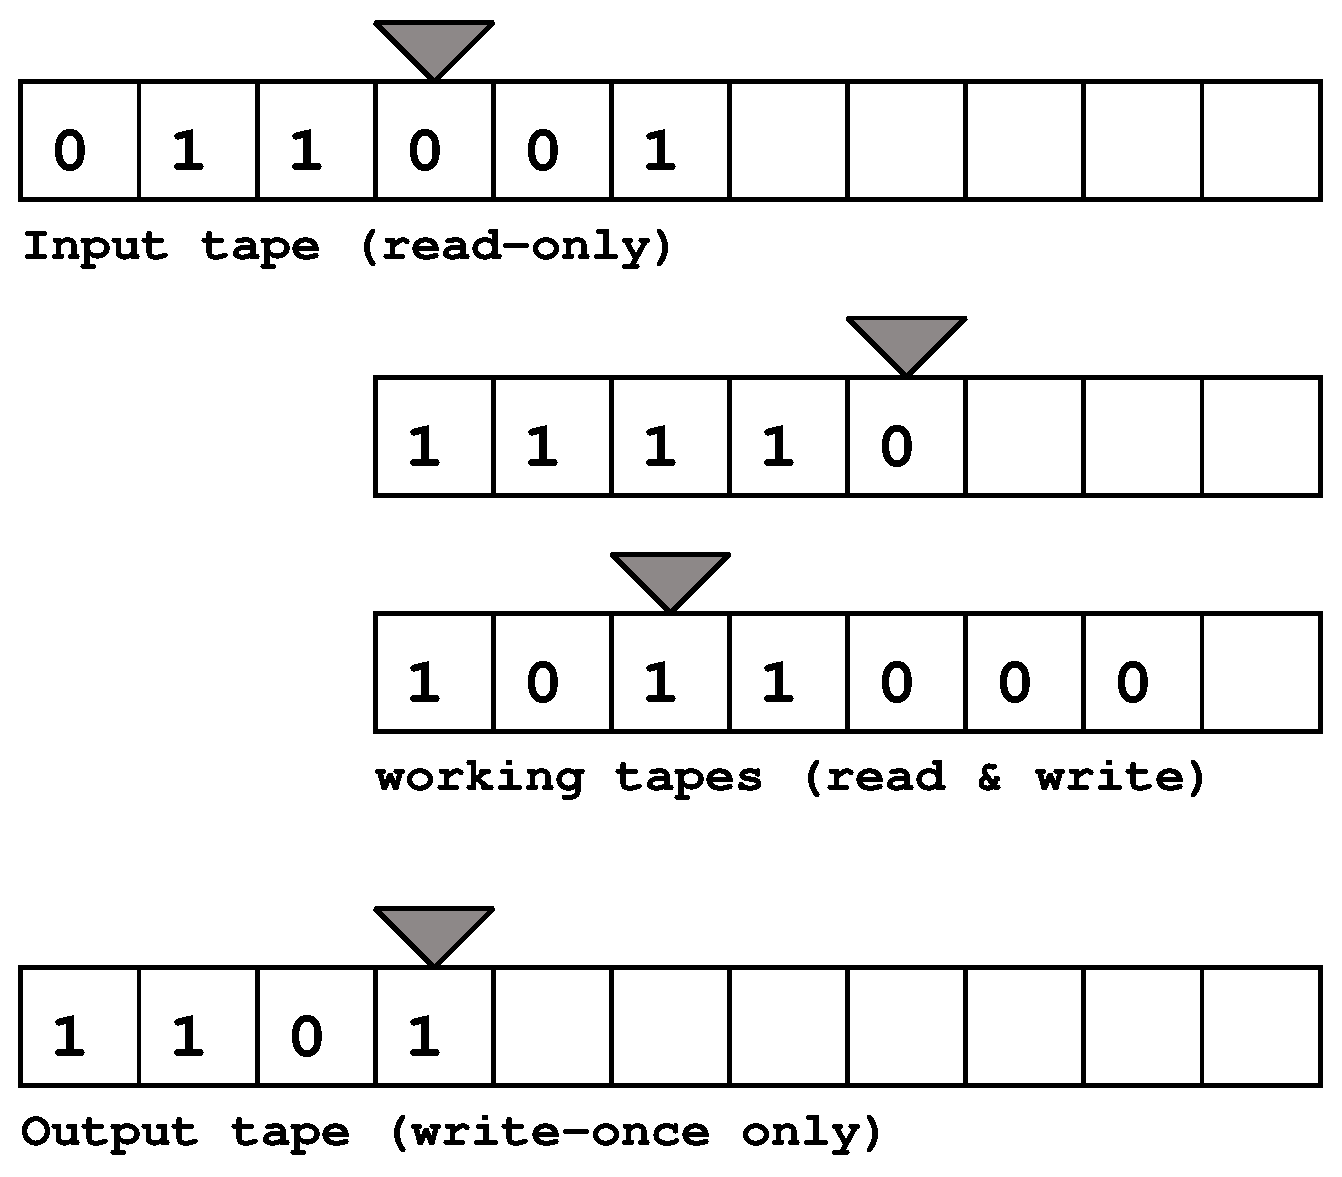
\includegraphics[width=0.5\textwidth]{turing_machine}
  \caption{A Turing machine operates with tapes}
  \label{fig:turing-machine}
\end{figure}

A \defemph{Turing machine} is a device which operates on a number of tapes and
heads, see \cref{fig:turing-machine}:
%
\begin{itemize}
\item a \defemph{read-only input tape} is equipped with a reading head that can move left and right, and read the symbols, but cannot write them.
\item The \defemph{read-write working tapes} are equipped with heads that move left and right, and can both read and write symbols.
\item The \defemph{write-once output tape} is equipped with a head which can
  move left and right, and it can write into each cell \emph{at most once}.
  Once a cell is filled with a non-blank symbol all subsequent writes
  to it are ignored.
\end{itemize}
%
The tapes are infinite\sidenote{If you are worried about having actual
  infinite tapes in your room, note that at each step of the
  computation only a finite portion of tapes has been inspected. In
  this sense the tapes are \emph{potentially} infinite.} and contain
symbols from a given finite alphabet. A common choice for the alphabet
is $0$, $1$, and a special symbol `blank'. The machine manipulates the
contents of the tapes according to a \defemph{program}, which is a \emph{finite}
list of simple instructions that control the heads and the tapes. The
machine executes one instruction at a time in a sequential manner. It
may \defemph{terminate} after having executed finitely many computation
steps. If it does not terminate then it runs forever, in which case we
say that it \defemph{diverges}.

Our version of Turing machine is different from the usual one, where a
machine is equipped with only a single tape that serves for input,
output, and intermediate work. The two formulations are equivalent in
the sense that a single-tape machine can simulate the workings of a
Turing machine with several tapes, and vice versa. Having working tapes will
ease the description of infinite computations in \cref{sec:type-2}.

The state of a Turing machine may be encoded onto a single tape as
follows. First we write down the program, suitably encoded by the
symbols from the alphabet, then the current state (the next
instruction to be executed), and positions of the heads. Finally, we
copy the contents of all the tapes by interleaving them into a single
tape.

If we were going to build just one machine, which one would we build?
The answer was given by Turing.

\begin{theorem}[Turing]
  \label{thm:universal-machine}
  There exists a \defemph{universal  machine}: a machine that takes a
  description of another machine, as explained above, and simulates
  it.
\end{theorem}

\begin{proof}
  A traditional proof may be found in any book on computability
  theory, and there is nothing wrong with reading the original
  proof~\sidecite{turing37:_comput_number_with_applic_to_entsc} either.
  For me a much more convincing proof is the fact that a universal
  machine is sitting right here on my desk. (You have to
    ignore the fact that several hundred gigabytes of storage are not
    quite the same thing as an infinite tape. Also, modern computers
    are really \emph{Von Neumann}
    machines~\sidecite{goldstein47:_repor_mathem_and_logic_aspec} because
    they have a central processing unit and random access memory
    instead of a tape.)
\end{proof}

Once we have a universal machine, we can make it behave like any other
machine. It is just
\href{http://www.catb.org/jargon/html/S/SMOP.html}{``a simple matter
  of programming''} to tell it what to do.

We mentioned in the introduction that many kinds of computing devices
are equivalent to Turing machines. We shall therefore not insist on
describing computation solely in terms of Turing machines, but rather
rely on familiarity with modern computers and programming languages.
After all, programs can actually be run on computers, whereas Turing
machines are hard to get by.


\subsection{Type 1 machines}
\label{sec:type-1}

How do we use Turing machines to compute a partial function $f :
\NN \parto \NN$? A natural idea is to write the argument $n$ onto the
input tape, run the machine until it terminates, and read the result
$f(n)$ off the output tape. If the machine diverges then $f(n)$ is
undefined. Of course, the input $n$ must be suitably encoded onto the
input tape, for example it can be written in binary form. The output
tape contains the result encoded in the same manner.

\begin{definition}
  A partial map $f : \NN \parto \NN$ is \defemph{computable} if there exists a Turing machine $M$ such that for every $n \in \NN$: if $f(n)$ is defined then~$M$ terminates on input~$n$ and gives output $f(n)$; if $f(n)$ is undefined then~$M$ diverges on input~$n$.
\end{definition}

It is convenient to view \emph{every} Turing machine as one computing a
function $\NN \parto \NN$. This can be arranged as long as we read the
result off the output tape correctly. Suppose the alphabet contains
symbols $0$, $1$, and blank. We encode the input $n$ onto the input
tape in binary followed by blanks, and run the machine. If and when it
terminates it has written at most finally many symbols onto the output
tape. Some of the symbols it has written might be different from $0$
and $1$. If we ignore everything that comes after the first blank, we
can interpret the output tape as a number written in binary (the empty
sequence encodes zero).

We can similarly define how a Turing machine computes a multivariate
partial function $f : \NN^k \parto \NN$. We just have to correctly
encode the arguments on the tape by placing special markers between
them so that we can tell where one ends and the next one begins.

\begin{exercise}
  Devise a coding scheme for $k$-tuples of numbers using the symbols $0$, $1$ and blank. Make sure that every tape which contains at most finitely many $0$'s and $1$'s encodes a $k$-tuple of numbers.
\end{exercise}

It is common knowledge that computers encode everything with $0$'s and~$1$'s, but logicians prefer to encode everything with natural numbers.
We shall write in general $\code{e}$ for \defemph{encoding} of $e$ by a natural
number. Of course, we must specify what $\code{e}$ is in each
particular case. For example, a pair of numbers $(m, n)$ may be
encoded into a single number as
%
\begin{equation*}
  \code{(m, n)} = 2^m (2 n + 1).
\end{equation*}
%
Every number except $0$ represents the code of a unique pair so we
also have computable \defemph{projections} $\xfst$ and $\xsnd$ which
recover $m$ and $n$ from $\code{(m, n)}$, respectively.
Once we know how to encode pairs of numbers, lists of numbers can be encoded as iterated pairs:
%
\begin{align*}
  \code{[\,]} &= 0 \\
  \code{[n_0, \ldots, n_k]} &= \code{(n_0, \code{[n_1, \ldots, n_k]})}.
\end{align*}
%
Because we defined $\code{(m,n)}$ so that it is never zero, the
elements of a sequence may be uniquely reconstructed from its code.
By iterating the scheme we may encode lists of lists of numbers, etc.

Turing machines can be encoded with numbers, also. A program is a finite
list of instructions, so it can be encoded as a finite sequence of
$0$'s and $1$'s (your computer does this every time you save a piece of
source code in a file), which in turn represents a number in binary
form. In fact, every number may be thought of as a code of a program
by the reverse process. Given a number, write it in binary form and
interpret it as a sequence of $0$'s and $1$'s and decode from it a
list of instructions. It may happen that the binary sequence does not
properly encode a list of instructions, in which case we interpret it
as some fixed silly little program.

The next step is to encode tapes and entire computations with numbers.
Because an infinite tape cannot be encoded in a single natural number,
we limit attention to the so-called \defemph{type 1 machines} which
accept only \emph{finite} inputs. More precisely, the input always
consists of a finite string of $0$'s and $1$'s followed by blanks.
Such input may be encoded by a single number. Furthermore, at every
step of computation the machine has used up only a finite portion of
its working tapes, whose contents may again be encoded by a single number.

By continuing in this manner we may encode with a single number a finite
sequence of computation steps, including the contents of the tapes
and positions of the heads at each step. Stephen Kleene~\sidecite{kleene43:_recur_predic_and_quant}
worked out the details of all this and defined the predicate
$T(x,y,z)$ whose meaning is
%
\begin{quote}
  ``Machine encoded by $x$ with input tape that encodes the number $y$
  performs a sequence of computation steps encoded by $z$ and
  terminates.''
\end{quote}
%
The amazing thing is that $T$ may be defined in \href{https://en.wikipedia.org/wiki/Peano_axioms#Peano_arithmetic_as_first-order_theory}{Peano arithmetic} just
in terms of $0$, successor, $+$ and $\times$. There is an
associated computable partial function $U(z)$ whose meaning is ``the
number encoded by the contents of the output tape in the last step of
computation encoded by $z$''. With it we can extract the result of a computation. It is easy to arrange $U$ so that it is defined for all~$z$, even those that do not encode terminating computations.

Kleene's normal form theorem~\sidecite{kleene43:_recur_predic_and_quant}
says that every partial computable function $f : \NN \parto \NN$ may
be written in the form
%
\begin{equation}
  \label{eq:kleene-normal-form}
  y \mapsto U(\min \set{z \in \NN \such T(x,y,z)}).
\end{equation}
%
The number $x$ is the encoding of a machine that computes~$f$. We
emphasize that we are completely ignoring questions of computational
efficiency. Just consider how we would compute $f(y)$ according
to~\eqref{eq:kleene-normal-form}: for each $z = 0, 1, 2, \ldots$, test
whether~$z$ encodes a computation of machine $x$ with input $y$. When
you find the first such~$z$, extract the result $U(z)$ from it. I dare
you to compute the identity function $y \mapsto y$ this way!

Kleene's normal form may be used to define a standard enumeration of
partial recursive functions. Let
%
\begin{equation*}
  \pr{x}{y} = U(\min \set{z \in \NN \such T(x,y,z)}).
\end{equation*}
%
The sequence $\xpr_0, \xpr_1, \xpr_2, \ldots$ is an enumeration of all
computable partial functions (with repetitions).

The preceding discussion may be generalized to functions of several
variables. For each $k \in \NN$ there is Kleene's predicate
$T^{(k)}(x,y_1,\ldots,y_k,z)$ and the corresponding $U^{(k)}(z)$ that
extracts results from computations. Similarly, there is a standard
enumeration of $k$-place computable partial functions
%
\begin{equation*}
  \prm{k}{x}{y_1, \ldots, y_k} =
  U^{(k)}(\min \set{z \in \NN \such T^{(k)}(x,y_1, \ldots, y_k,z)}).
\end{equation*}
%
These enumerations are not arbitrary, because they have the following
important properties.

\begin{theorem}[utm]
  There exists a partial computable function $u : \NN \times
  \NN \parto \NN$ such that, for all $x, y \in \NN$,
  %
  \begin{equation*}
    u(x,y) \simeq \pr{x}{y}.
  \end{equation*}
\end{theorem}

\begin{theorem}[smn]
  There exists a computable function $s :
  \NN^2 \to \NN$ such that, for all $x, y, z \in \NN$,
  %
  \begin{equation*}
    \pr{s(x, y)}{z} \simeq \prm{2}{x}{y,z}.
  \end{equation*}
\end{theorem}

\noindent
The utm theorem is essentially a restatement of
\cref{thm:universal-machine} in terms of computable partial
functions. Detailed proofs of the utm and smn theorems would involve
a lot of technical manipulations of Turing machines, you may consult~\sidecite{davis58:_comput_unsol} to get a taste of it.
It is illuminating to see how the utm and smn theorems manifest themselves in modern programming languages, say in Haskell. Keeping in mind that numbers are just codes for programs and data, the universal function $u$ from the utm theorem is
%
\begin{lstlisting}[language=Haskell]
u (f, y) = f y
\end{lstlisting}
%
and the function $s$ is the currying operation\sidenote{In Haskell the
  notation \texttt{{\char92}x -> e} stands for $\lambda$-abstraction
  $\lam{x}{e}$, which in turn means ``the function which maps $x$ to
  $e$'', see \cref{sec:lambda-calculus}.}
%
\begin{lstlisting}[language=Haskell]
s (f, y) = \z -> f (y, z)
\end{lstlisting}
%
This may seem like a triviality to the programmer but is surely not
considered one by the implementors of the Haskell compiler. The definition of \lstinline!s! uses function application, pairing, currying and $\lambda$-abstraction, which are ``the essence'' of functional programming, just like the utm and smn theorems are the essence of partial computable functions.

The following theorem is important in the theory of computable
functions because it allows us to define partial computable functions
by recursion.

\begin{theorem}[Recursion theorem]
  For every \emph{total} computable $f : \NN \to \NN$ there exists $n
  \in \NN$ such that $\xpr_{f(n)} = \xpr_{n}$.
\end{theorem}

\begin{proof}
  The classical proof goes as follows. First we define a computable
  partial map $\psi : \NN^2 \parto \NN$ such that
  %
  \begin{equation*}
    \psi(u, x) = \pr{\pr{u}{u}}{x},
  \end{equation*}
  %
  where $\psi(u, x)$ is undefined when $\pr{u}{u}$ is undefined.
  %
  By the smn theorem there is a computable function $g : \NN \to \NN$
  such that $\pr{g(u)}{x} = \psi(u, x)$. Now consider any computable
  $f : \NN \to \NN$. Because $f \circ g$ is computable, there exists
  $v \in \NN$ such that $\xpr_{v} = f \circ g$. Since $f \circ g$ is a
  total function, $\pr{v}{v}$ is defined. The number $n = g(v)$ has
  the desired property:
  $\xpr_{g(v)} = \xpr_{\pr{v}{v}} = \xpr_{f(g(v))} = \xpr_{f(n)}$.
\end{proof}

This was a typical argument in the theory of computable functions. Let
us prove the recursion theorem in Haskell to see what is going on. The
function $f : \NN \to \NN$ operates on codes of computable partial
maps. Haskell has higher-order functions that work directly with functions as arguments and results, so $f$ should be given the type
%
\begin{lstlisting}[language=Haskell]
f :: (Integer -> Integer) -> (Integer -> Integer)
\end{lstlisting}
%
Rather than looking for a number $n$ we are looking for a function
%
\begin{lstlisting}[language=Haskell]
n :: Integer -> Integer
\end{lstlisting}
%
such that \lstinline!f n = n!. Because Haskell already has recursion built in this is very easy, just define
%
\begin{lstlisting}
n = f n
\end{lstlisting}
%
The Recursion theorem is nothing but definition by recursion for type~1 machines.

We finish this section with a theorem which we shall often use to show
\emph{non}-computability results.

\begin{theorem}[Halting oracle]
  The \defemph{halting oracle},
  %
  \begin{equation*}
    h(x) =
    \begin{cases}
      1 & \text{if $\pr{x}{0}$ is defined,}\\
      0 & \text{if $\pr{x}{0}$ is not defined,}
    \end{cases}
  \end{equation*}
  %
  is \emph{not} computable.
\end{theorem}

\begin{proof}
  Let us prove the theorem in Haskell. We must show that there is no
  %
\begin{lstlisting}[language=Haskell]
h :: (Integer -> Integer) -> Integer
\end{lstlisting}
  %
  such that, for all \lstinline!f :: Integer -> Integer!,
  %
  \begin{equation*}
    \text{\lstinline!h f!} =
    \begin{cases}
      \text{\lstinline!1!} & \text{if \lstinline!f 0! terminates,}\\
      \text{\lstinline!0!} & \text{if \lstinline!f 0! diverges.}
    \end{cases}
  \end{equation*}
  %
  Suppose there were such an \lstinline!h!. Define
  %
\begin{lstlisting}[language=Haskell]
g n = if h g == 1 then g n else 0
\end{lstlisting}
  %
  By assumption \lstinline!h g! is either \lstinline!0! or
  \lstinline!1!. In either case there is a contradiction because
  \lstinline!g! does just the opposite of what \lstinline!h! says it
  will do.
\end{proof}

\subsection{Type 2 machines}
\label{sec:type-2}

Type 1 machines from previous section only operate on finite inputs.
In practice we often see programs whose input and output are
(potentially) infinite. For example, when you listen to an Internet
radio station, the player accepts a never-ending stream of data which
it outputs to the speakers. Also, many useful programs, such as servers, operating systems, and browsers are potentially non-terminating. We therefore need a model of computation that describes non-terminating programs with infinite inputs and outputs.

A popular one is \defemph{type 2 machine}, which accepts an
infinite sequence on its input tape and is allowed to work forever. It
may or may not fill the output tape entirely with non-blank symbols.
Note that the requirement for the output tape to be write-once makes
it possible to tell when the machine has actually produced an output
in a given cell. Had we allowed the machine to write to each output
cell many times, it could keep coming back and changing what it has
already written.

An important distinction between type 1 and type 2 machines is that
the latter may accept non-computable inputs, from which non-computable
outputs may be produced.

For type 2 machines there are analogues of the standard
enumeration~$\xpr$, utm and the smn theorems. These are more easily
expressed if we allow the machines to write natural numbers in the
cells, rather than symbols from a finite alphabet. We also equip the
machines with instructions for manipulating numbers, say, instructions
for extracting the bits and for testing equality with zero. These
changes are inessential because an infinite sequence $n_0, n_1, n_2,
\ldots$ of natural numbers may be encoded as a binary sequence
$1^{n_0}01^{n_1}01^{n_2}0\cdots$, where $1^k$ means that the symbol
$1$ is repeated $k$-times.

\begin{definition}
  Say that a type 2 machine $M$ \textbf{computes} a partial map $f : \NNNN \parto
  \NNNN$ when for every $\alpha \in \NNNN$:
  %
  if $f(\alpha)$ is defined then~$M$ eventually writes to every output cell, and the output tape equals $f(\alpha)$; if $f(\alpha)$ is not defined, then at least one output cell to which~$M$ never writes to.

  A partial map $f : \NNNN \parto \NNNN$ is \textbf{type~2 computable} if it is computed by a type~2 machine.
\end{definition}

We may similarly define what it means for a machine to compute a multivariate partial function $f : (\NNNN)^k \parto \NNNN$. The input $(\alpha_0, \ldots, \alpha_{k-1})$ is written onto the input tape in an interleaving manner, so that $\alpha_i(j)$ is found in the cell at position $k \cdot j + i$.

\subsubsection{The Baire space}
\label{sec:baire-space}

We recall a few basic facts about the \defemph{Baire space~$\Baire = \NNNN$}. Let $\NN^{*}$ be the set of all finite sequences of natural numbers. If $a, b \in \NN^{*}$
we write $a \sqsubseteq b$ when $a$ is a prefix of~$b$. The length of a finite sequence $a$ is denoted by~$\T{a}$. Similarly, we write $a \sqsubseteq \alpha$ when $a$ is a prefix of an infinite sequence $\alpha \in \Baire$. Define $\seg{a}{n} = [\alpha(0), \ldots,
\alpha(n-1)]$ to be the prefix of~$\alpha$ consisting of the first~$n$ terms.

Write $\cons{n}{\alpha}$ for the sequence $n, \alpha(0), \alpha(1), \alpha(2), \ldots$, and $\append{a}{\beta}$ for concatenation of the finite sequence $a \in \NN^{*}$ with the infinite sequence $\beta \in \Baire$.

We equip $\Baire$ with the product topology, which is the topology whose countable topological base consists of the basic open sets, for $a \in \NN^{*}$,
%
\begin{equation*}
  \basicBB{a}
  = \set{\append{a}{\beta} \such \beta \in \Baire}
  = \set{\alpha \in \Baire \such a \sqsubseteq \alpha}.
\end{equation*}
%
Because the basic open sets are both closed and open (clopen),
$\Baire$ is in fact a countably based $0$-dimensional\sidenote{Recall
  that a space is \defemph{$0$-dimensional} when its clopen subsets form
  a base for its topology.} Hausdorff space. It is also a complete
separable metric space for the \defemph{comparison metric} $d : \Baire
\times \Baire \to \RR$, defined by
%
\begin{equation*}
  d(\alpha, \beta) = \inf \,\set{2^{-n} \such
    \seg{\alpha}{n} = \seg{\beta}{n}}.
\end{equation*}
%
If the first term in which $\alpha$ and $\beta$ differ is the $n$-th
one, then $d(\alpha, \beta) = 2^{-n}$. The comparison metric is an
\defemph{ultrametric}, which means that it satisfies the inequality $d(\alpha,
\gamma) \leq \max(d(\alpha, \beta), d(\beta, \gamma))$. In an ultrametric space every point of a ball is its center. The clopen sets $\basicBB{a}$ are precisely the balls of radius $2^{-\T{a}}$.

\subsubsection{Encoding of partial maps $\Baire \parto \Baire$}
\label{sec:encoding-maps-baire}

Earlier we encoded the partial computable maps $\NN \parto \NN$ with numbers describing Turing machines. We would like to similarly encode computable partial maps $\Baire \parto \Baire$ with sequences. An obvious idea, which we shall not pursue, is to use the first term of a sequence to encode a Turing machine. Instead, we shall use sequences as ``lookup tables'', with which even some non-computable maps will be encoded.

Consider a partial map $f : \Baire \parto \Baire$ computed by~$M$.
Suppose that, given an input tape
%
\begin{equation*}
  \alpha = n_0, n_1, n_2, \ldots
\end{equation*}
%
$M$~writes $j$ to the $i$-th output cell after $k$~steps of computation,
hence $f(\alpha)(i) = j$. Because in~$k$ steps~$M$ inspects at most the first $k$ input cells, it would have done the same for any other input that agrees with the given one in the first~$k$ terms. Thus $f$ is determined by pieces of information of the form:
%
\begin{quote}
  ``If the input starts with $n_0, n_1, \ldots, n_{k-1}$ then the $i$-th term of the output is~$j$.''
\end{quote}
%
A code~$\gamma \in \Baire$ of~$f$ just has to contain such information, which we can arrange by coding lists and pairs as numbers. To determine the value $\gamma(m)$ for a given $m \in \NN$, decode~$m + 1$ as a finite sequence $m + 1 = \seq{i, n_0, \ldots, n_{k-1}}$ and simulate~$M$ for~$k$ steps with the input tape
%
\begin{equation*}
  n_0, \ldots, n_{k-1}, 0, 0, \ldots
\end{equation*}
%
If the machine writes $j$ into the $i$-th output cell during the simulation, set $\gamma(m) = j + 1$, otherwise set $\gamma(m) = 0$.
%
Think of $\gamma$ as a lookup table which maps a key $\cons{i}[n_0, \ldots, n_{k-}]$ to an optional value~$j$.
%
Clearly, $\gamma$ can be computed from a description of~$M$.

To decode the function $\xfpr_\gamma : \Baire \parto \Baire$ encoded by $\gamma \in \Baire$, we just have to devise a lookup procedure. Given input $\alpha \in \Baire$, we compute the value of the $i$-th output cell by successively looking up keys $\cons{i}{\seg{\alpha}{k}}$ for ever larger~$k$, until we find an answer~$j$. More precisely,
for $\alpha \in \Baire$, define $\ell(\gamma, \alpha) : \NN \parto \NN$ as
%
\begin{equation*}
  \ell(\gamma, \alpha)(i) = \gamma(\code{\cons{i}{\seg{\alpha}{k}}}) - 1
  \quad\text{where}\quad
  k = \min\nolimits_k (\gamma(\code{\cons{i}{\seg{\alpha}{k}}}) \neq 0)
\end{equation*}
%
(if not such $k$ exists then $\ell(\gamma, \alpha)(i)$ is undefined), and let the map $\xfpr_\gamma : \Baire \parto \Baire$ encoded by $\gamma$ be
%
\begin{equation}
  \label{eq:type2-encoding}
  \fpr{\gamma}{\alpha} =
  \begin{cases}
    \ell(\gamma, \alpha) & \text{if $\ell(\gamma, \alpha)$ is a total map,} \\
    \text{undefined} & \text{otherwise.}
  \end{cases}
\end{equation}

\begin{definition}
  \label{def:type-2-realized}%
  A partial function $f : \Baire \parto \Baire$ is \defemph{(type 2) realized} by $\gamma \in \Baire$, called a \defemph{Kleene associate} of~$f$, when $f = \xfpr_\gamma$.
\end{definition}

Clearly, if $\gamma$ is a computable sequence then $\xfpr_\gamma$ is type 2 computable.
But what sort of partial map is $\xfpr_\gamma$ in general?

An arbitrary $\gamma \in \Baire$ may give inconsistent answers, in the sense that looking up values at $\cons{i}{\seg{\alpha}{k}}$ and $\cons{i}{\seg{\alpha}{m}}$ may give inconsistent answers. Above we resolved the problem by taking the answer given by the least~$k$. We may also rectify~$\gamma$ to a realizer that gives consistent answers.

Say that $\gamma \in \Baire$ is \defemph{consistent} when, for all $k, m \in \NN$ and
$\alpha \in \Baire$, if $k < m$ and $\gamma(\code{\seg{\alpha}{k}}) \neq 0$ then
$\gamma(\code{\seg{\alpha}{m}}) = \gamma(\code{\seg{\alpha}{k}})$.

\begin{lemma}
  \label{lemma:normalized-BB}%
  Every realized function is realized by a consistent realizer.
\end{lemma}

\begin{proof}
  Suppose $f : \Baire \parto \Baire$ is realized by~$\gamma$. Define
  $\delta$ by induction on the length of $a \in \NN^{\star}$ by
  %
  \begin{equation*}
    \delta(\code{a}) =
    \begin{cases}
      \gamma(\code{a}) & \text{if $a = [\,]$,}\\
      \gamma(\code{a}) & \text{if $a = \cons{i}{a'}$ and
        $\delta(\code{a'}) = 0$,}\\
      \delta(\code{a'}) & \text{if $a = \cons{i}{a'}$ and
        $\delta(\code{a'}) \neq 0$,}
    \end{cases}
  \end{equation*}
  %
  The realizer $\delta$ is consistent by construction. It is easy to check that $\xfpr_\gamma = \xfpr_\delta$.
\end{proof}

\begin{theorem}[Extension Theorem for $\Baire$]%
  \label[extensionTheorem]{th:extension_BB}%
  Every partial continuous map $f: \Baire \parto \Baire$ can be extended
  to a realized one.
\end{theorem}

\begin{proof}
  Suppose $f: \Baire \parto \Baire$ is a partial continuous map, and let
  %
  \begin{align*}
     A = \big\{ & (a, i, j) \in \NN^{*} \times \NN^{2} \such \\
       &\basicBB{a} \cap \dom{f} \neq \emptyset \land
        \all{\alpha}{(\basicBB{a} \cap \dom{f})}{
          f(\alpha)(i) = j
          }
        \big\}.
  \end{align*}
  %
  If $(a, i, j) \in A$ and $(a', i, j') \in A$ and $a \sqsubseteq a'$
  then $j = j'$ because there is $\alpha \in \basicBB{a'} \cap
  \dom{f} \subseteq \basicBB{a} \cap \dom{f}$ such that $j =
  f(\alpha)(i) = j'$. We define a sequence $\gamma \in \Baire$ as
  follows. For every $(a, i, j) \in A$ let
  $\gamma(\code{\cons{i}{a}}) = j + 1$, and for all other
  arguments $n$ let $\gamma(n) = 0$. Suppose that
  $\gamma(\code{\cons{i}{a}}) = j + 1$ for some $i, j \in \NN$
  and $a \in \NN^{*}$. Then for every prefix $a' \sqsubseteq a$,
  $\gamma(\code{\cons{i}{a'}}) = 0$ or
  $\gamma(\code{\cons{i}{a'}}) = j + 1$. Thus, if $(a, i, j) \in
  A$ and $a \sqsubseteq \alpha$ then $\fpr{\gamma}{\alpha}(i) = j$.
  %
  Let us how that $\fpr{\gamma}{\alpha}(i) = f(\alpha)(i)$ for all
  $\alpha \in \dom{f}$ and all $i \in \NN$. Because~$f$ is continuous,
  for all $\alpha \in \dom{f}$ and $i \in \NN$ there exists $(a, i, j)
  \in A$ such that $a \sqsubseteq \alpha$ and $f(\alpha)(i) = j$. Now
  we get
  %
  $
    \fpr{\gamma}{\alpha}(i)
    = j
    = f(\alpha)(i)
  $.
\end{proof}

\index{set!G-delta set@{$G_\delta$}}%
Recall that a \defemph{$G_\delta$-set} is a countable intersection of open sets.

\begin{lemma}
  \label{th:G_delta_characteristic}%
  If $U \subseteq \Baire$ is a $G_\delta$-set then the partial
  function $u: \Baire \parto \Baire$, defined by
  %
  \begin{equation*}
    u(\alpha) =
    \begin{cases}
      1 & \text{if $\alpha \in U$.}\\
      \text{undefined} & \text{otherwise,}
    \end{cases}
  \end{equation*}
  %
  is realized.
\end{lemma}

\begin{proof}
  The set $U$ may be expressed as a countable intersection of countable unions of basic
  open sets,
  %
  \begin{equation*}
    U = \bigcap_{i \in \NN}
        \bigcup_{j \in \NN} \basicBB{a_{i,j}}.
  \end{equation*}
  %
  Define $\gamma \in \Baire$ by setting
  $\gamma(\code{\cons{i}{a_{i,j}}}) = 2$ for all $i, j \in \NN$,
  and $\gamma(n) = 0$ for all other arguments~$n$. Clearly, if
  $\fpr{\gamma}{\alpha}$ is defined then its value is the constant
  sequence $1, 1, 1, \ldots$, so we only need to verify that
  $\dom{\xfpr_\gamma} = U$. If $\alpha \in \dom{\xfpr_\gamma}$ then
  $\ell(\gamma,\alpha)(i)$ is defined for every $i \in \NN$.
  For every $i \in \NN$ there exists $j_i \in \NN$ such that $\gamma
  (\code{\cons{i}{\seg{\alpha}{j_i}}}) = 2$, which implies that $
  a_{i, j_i} \sqsubseteq \alpha$. Hence
  %
  \begin{equation*}
    \alpha \in \bigcap_{i \in \NN} \basicBB{a_{i, j_i}} \subseteq U.
  \end{equation*}
  %
  Conversely, suppose $\alpha \in U$ and consider any $i \in \NN$.
  There exists $j \in \NN$ such that $a_{i,j} \sqsubseteq \alpha$,
  therefore $\gamma (\code{\cons{i}{\seg{\alpha}{|a_{i,j}|}}}) =
  \gamma(\code{\cons{i}{a_{i,j}}}) = 2$ so that $\ell(\gamma,\alpha)(i)$ is defined. We conclude that $\alpha \in
  \dom{\xfpr_\gamma}$.
\end{proof}

\begin{lemma}
  \label{th:restrict_G_delta}%
  Suppose $\alpha \in \Baire$ and $U \subseteq \Baire$ is a $G_\delta$-set.
  Then there exists $\delta \in \Baire$ such that
  %
  $\dom{\xfpr_\delta} = U \cap \dom{\xfpr_\alpha}$
  %
  and
  %
  $\fpr{\alpha}{\beta} = \fpr{\delta}{\beta}$
  %
  for all $\beta \in \dom{\xfpr_\alpha} \cap U$.
\end{lemma}

\begin{proof}
  By \cref{lemma:normalized-BB} we may assume that $\alpha$ is normalized.
  Define $f: \Baire \parto \Baire$ by
  %
  \begin{equation*}
    f(\beta)(n) =
    \begin{cases}
      \fpr{\alpha}{\beta}(n) &
      \text{if $\beta \in \dom{\xfpr_\alpha} \cap U$,} \\
      \text{undefined} & \text{otherwise}
    \end{cases}
  \end{equation*}
  %
  We would like to show that $f$ is realized. From \cref{th:G_delta_characteristic} we obtain a normalized $\gamma \in \Baire$ such that, for all $\beta \in \Baire$,
  %
  \begin{equation*}
    \fpr{\gamma} \beta =
    \begin{cases}
      \lam{n}{1} & \beta \in U,\\
      \text{undefined} & \text{otherwise}.
    \end{cases}
  \end{equation*}
  %
  We claim that $f$ is realized by
  %
  \begin{equation*}
    \delta(k) = \alpha(k) \cdot \gamma(k)/2.
  \end{equation*}
  %
  Recall that $\gamma(k)$ is either $0$ or $2$ so $\delta(k)$ is
  either $0$ or $\alpha(k)$. Hence $\xfpr_\delta$ is a restriction of
  $\xfpr_\alpha$, by which we mean that $\dom{\xfpr_\delta} \subseteq
  \dom{\xfpr_\alpha}$ and $\fpr{\delta}{\beta} = \fpr{\alpha}{\beta}$
  for all $\beta \in \dom{\xfpr_\delta}$. Also, $\dom{\xfpr_\delta}
  \subseteq \dom{\xfpr_\gamma}$ because $\delta(k) \neq 0$ implies
  $\gamma(k) \neq 0$. It remains to be shown that $\beta \in
  \dom{\xfpr_\alpha} \cap U$ implies $\beta \in \dom{\xfpr_\delta}$,
  i.e., that for such $\beta$, $\ell(\delta, \beta)(i)$ is
  defined for every $i \in \NN$. Because $\ell(\alpha, \beta)(i)$
  and $\ell(\gamma, \beta)(i)$ are
  defined, there exist $k_1$ and $k_2$ such that
  %
  \begin{equation*}
    \alpha(\code{\cons{i}{\seg{\beta}}{k_1}}) \neq 0
    \qquad\text{and}\qquad
    \gamma(\code{\cons{i}{\seg{\beta}}{k_2}}) \neq 0.
  \end{equation*}
  %
  Because $\alpha$ and $\gamma$ are normalized, for $k = \max(k_1,
  k_2)$,
  %
  \begin{equation*}
    \alpha(\code{\cons{i}{\seg{\beta}}{k}}) \neq 0
    \qquad\text{and}\qquad
    \gamma(\code{\cons{i}{\seg{\beta}}{k}}) \neq 0,
  \end{equation*}
  %
  hence $\delta(\code{\cons{i}{\seg{\beta}}{k}}) \neq 0$, which we
  wanted to show.
\end{proof}

We are now able to characterize the realized maps.

\begin{theorem}
  A partial function $f: \Baire \parto \Baire$ is realized if, and only
  if, $f$ is continuous and its support is a $G_\delta$-set.
\end{theorem}

\begin{proof}
  First we show that $\xfpr_\alpha$ is a continuous map whose support
  is a $G_\delta$-set. It is continuous because the value of
  $\fpr{\alpha}{\beta}(n)$ depends only on $n$ and a finite prefix of
  $\beta$. The support of $\xfpr_\alpha$ is the $G_\delta$-set
  %
  \begin{align*}
    \dom{\xfpr_\alpha}
    &= \set{\beta \in \Baire \such
      \all{n}{\NN}{
        \ell(\alpha, \beta)(n) \ \text{defined and $> 0$}}} \\
    &= \tbigcap_{n \in \NN}
      \set{\beta \in \Baire \such
        \ell(\alpha, \beta)(n) \ \text{defined and $> 0$}} \\
    &=  \tbigcap_{n \in \NN}
        \tbigcup_{m \in \NN}
          \set{\beta \in \Baire \such
          \ell(\alpha, \beta)(n) = m + 1}.
  \end{align*}
  %
  Each of the sets $\set{\beta \in \Baire \such \ell(\alpha, \beta)(n) = m}$ is open because~$\ell$ is a continuous operation.
  
  Now let $f: \Baire \parto \Baire$ be a partial continuous function
  whose support is a $G_\delta$-set. By \cref{th:extension_BB}
  there exists $\gamma \in \Baire$ such that $f(\alpha) =
  \fpr{\gamma}{\alpha}$ for all $\alpha \in \dom{f}$. By
  \cref{th:restrict_G_delta} there exists $\psi \in \Baire$ such
  that $\dom{\xfpr_\psi} = \dom{f}$ and $\fpr{\psi}{\alpha} =
  \fpr{\gamma}{\alpha}$ for every $\alpha \in \dom{f}$.
\end{proof}

Finally, we formulate the utm and smn theorems for type 2 machines.

\begin{theorem}[type 2 utm]
  \label{th:type-2-utm}%
  There exists a computable partial function $u : \Baire \times
  \Baire \parto \Baire$ such that $u(\alpha, \beta) \simeq
  \fpr{\alpha}{\beta}$ for all $\alpha, \beta \in \Baire$.
\end{theorem}

\begin{proof}
  Let us write a machine for computing $u$ in Haskell, but without
  resorting to an explicit encoding of finite sequences by numbers.
  Define the type
  %
\begin{lstlisting}
type Baire = Integer -> Integer
\end{lstlisting}
  %
  The universal \lstinline!u :: ([Integer] -> Integer, Baire) -> Baire! %
  is just the transliteration of~\eqref{eq:type2-encoding}:
  %
\begin{lstlisting}[language=Haskell]
u (a, b) i = x - 1
    where x = head $
              filter (/= 0) $
              [a (i : map b [0..(k-1)]) | k <- [0..]]
\end{lstlisting}
  % 
  You may entertain yourself by learning Haskell and figuring out how
  it works.
\end{proof}

The type 2 variant of the smn theorem uses the representation
$\xfpr^{(2)}$ for encoding partial maps $\Baire \times \Baire \to
\Baire$ by
%
\begin{equation*}
  \fprm{2}{\alpha}{\beta, \gamma} = \fpr{\alpha}{\pair{\beta, \gamma}}
\end{equation*}
%
where $\pair{\beta, \gamma}$ is the interleaved sequence $\beta(0), \gamma(0), \beta(1), \gamma(1), \ldots$.

\begin{theorem}[type 2 smn]
  \label{th:type-2-smd}%
  There exists a computable $s : \Baire \times \Baire \to \Baire$ such
  that, for all $\alpha, \beta, \gamma \in \Baire$,
  %
  \begin{equation*}
    \fpr{s(\alpha, \beta)}{\gamma} = \fprm{2}{\alpha}{\beta, \gamma}.
  \end{equation*}
\end{theorem}

\begin{proof}
  Exercise in Haskell programming.
\end{proof}

%%%%%%%%%%%%%%%%%%%%%%%%%%%%%%%%%%%%%%%%%%%%%%%%%%
\subsection{Turing machines with oracles}
\label{sec:turing-machines-with}

The computational models from \Cref{sec:type-1}\ref{sec:type-2} \emph{relativize}, i.e.,
they may be adapted to use \defemph{oracle Turing machines}. Recall that an \defemph{oracle} is an infinite binary sequence $\omega : \NN \to \set{0, 1}$ and that a Turing machine with oracle~$\omega$ is a Turing machine with an extra read-only tape containing~$\omega$. The machine consults the tape to obtain the values of~$\omega$.
When $\omega$ is a non-computable sequence, the oracle machine exceedds the computational power of ordinary Turing machines.

Each oracle $\omega$ yields a type 1 and a type 2 model of computation in which the machines have access to~$\omega$. That is, in any given such model all machines access the same fixed oracle~$\omega$.


%%%%%%%%%%%%%%%%%%%%%%%%%%%%%%%%%%%%%%%%%%%%%%%%%%
\subsection{Hamkin's infinite-time Turing machines}
\label{sec:iitm}

Another model of computation that exceeds the power of Turing machines are Hamkin's \defemph{infinite-time Turing machines}~\sidecite{hamkins00:_infin_turin}. We give here just a brief overview and recommend the cited reference for background reading.

An infinite-time Turing machine, or just \emph{machine}, is like a Turing
machine which is allowed to run infinitely long, with the computation steps
counted by ordinal numbers. The machine has a finite program, an input tape, work
tapes, an output tape, etc. We assume that the tape cells contain $0$'s and
$1$'s. At successor ordinals the machine acts like an ordinary Turing machine.
At limit ordinals it enters a special ``limit'' state, its heads are placed at
the beginnings of the tapes, and the content of each tape cell is computed as
the $\limsup$ of the values written in the cell at earlier stages. More
precisely, if $c_\alpha$ denotes the value of the cell $c$ at step $\alpha$,
then for a limit ordinal $\beta$ we have
%
\begin{equation*}
  c_\beta =
  \begin{cases}
    0 & \text{if $\some{\alpha < \beta} \all{\gamma}
      (\alpha \leq \gamma < \beta \Rightarrow c_\alpha = 0)$},\\
    1 & \text{otherwise}.
  \end{cases}
\end{equation*}
%
The machine terminates by entering a special halt state, or it may run forever. It turns
out that a machine which has not terminated by step $\omega_1$ runs forever.

We can think of machines as computing partial functions $\Cantor \parto \Cantor$ where $\two = \set{0, 1}$:
%
initialize the input tape with an infinite binary sequence $x \in \Cantor$, run the
machine, and observe the contents of the output tape if and when the machine terminates.
We can also consider infinite time computation of partial functions $\NN \parto \NN$:
initialize the input tape with the input number, run the machine, and interpret the
contents of the output tape as a natural number, where we ignore anything that is beyond
the position of the output head. By performing the usual encoding tricks, we can feed the
machines more complicated inputs and outputs, such as pairs, finite lists, and even
infinite lists of numbers. We say that a function is \defemph{infinite-time computable} if there is an infinite-time Turing machine that computes it.

The power of infinite-time Turing machines is vast and extends far beyond the halting
problem for ordinary Turing machines, although of course they cannot solve their own
halting problem. For example, for every $\Pi^1_1$-subset $S \subseteq \Cantor$ there is a machine which, given $x \in \Cantor$ on its input tape, terminates and decides whether $x \in S$.

There is a standard enumeration $M_0, M_1, M_2, \ldots$ of infinite-time Turing
machines, where $M_n$ is the machine whose program is encoded by the number $n$
in some reasonable manner. The associated enumeration $\iitm{0}, \iitm{1}, \iitm{2},
\ldots$ of infinite-time computable partial functions $\NN \parto \NN$ is
defined as
%
\begin{equation*}
  \iitm{n}(k) =
  \begin{cases}
    m & \text{if $M_n(k)$ terminates and outputs $m$,}\\
    \text{undefined} & \text{otherwise}.
  \end{cases}
\end{equation*}
%
We may similarly an enumeration $\iitm{0}^{(k)}, \iitm{1}^{(k)}, \iitm{2}^{(k)}, \ldots$ of $k$-ary infinite-time computable partial maps $\NN^k \parto \NN$.

The enumeration satisfies the smn and utm theorems.

\begin{theorem}[infinite-time smn]
  There is an infinite time computable total map $s : \NN \times \NN \to \NN$
  such that $\iitm{{s}(m,n)}(j) = \iitm{m}^{(2)}(n, j)$ for all $m, n, j \in \NN$.
\end{theorem}

\begin{theorem}[infinite-time utm]
  There is an infinite-time computable partial map $u : \NN \times \NN \parto
  \NN$ such that $\iitm{t}(m) = u(t,m)$ for all $t, m \in \NN$.
\end{theorem}

\noindent
%
To convince ourselves that the utm theorem holds, we think a bit how a universal
infinite-time Turing machine works. It accepts the description~$n$ of a machine and the
initial input tape~$x$. At successor steps the simulation of machine~$M_n$ on input~$x$
proceeds much like it does for the ordinary Turing machines. Thus it takes finitely many
successor steps to simulate one successor step of $M_n$. Each limit step of $M_n$ is
simulated by one limit step of the universal machine, followed by finitely many successor
steps. Indeed, whenever the universal machine finds itself in the special limit state, it
puts the simulated machine in the simulated limit state, and moves the simulated heads to
the beginnings of the simulated tapes. These actions take finitely many steps. The
contents of the simulated tapes need not be worried about, as it will be updated correctly at limit stages.

To see what sort of tasks can be performed by infinite-time Turing machines, we consider
several examples that will be useful later on.

\begin{example}
  There is a machine which decides whether two infinite sequences $x, y \in
  \Cantor$ are equal. It first initializes a fresh work cell with~$0$, and then
  for each~$k$, it compares $x(k)$ and $y(k)$. If they differ, it sets the work cell to~$1$. After $\omega$ steps the work cell will be $1$ if, and only if, $x \neq y$.
\end{example}

\begin{example}
  A more complicated problem is to \emph{semi}decide whether a given machine $M_n$ computes
  a given sequence $x \in \Cantor$. The machine which performs such a task accepts $n$ and $x$ as inputs and begins by writing down the sequence $y_k = \iitm{n}(k)$ onto a work tape. This it can do by simulating $M_n$ successively on inputs $0, 1, 2, \ldots$ and writing down the values $y_k$ as they are obtained. The machine also keeps track for which~$k$'s the values $y_k$ have been computed by flipping the $k$-th bit of a separate ``tally'' tape from $0$ to $1$ whenever $M_n(k)$ terminates. If any of the $y_k$'s is undefined, the machine will run forever. Otherwise it will be able to detect in $\omega$ steps that the entire sequence $y$ has been computed and written down by checking that all bits on the separate ``tally'' tape have been flipped to~$1$. After that, the machine verifies that $x_k = y_k$ for all $k \in \NN$, as described previously.
\end{example}

\begin{example}
  Suppose we have a machine~$M$ which expects as input an infinite sequence~$x$ and a
  number~$n$. We would like to construct another machine which accepts an infinite
  sequence~$x$ and outputs a number~$n$ such that $M(x,n)$ terminates, if one exists.
  We use the familiar dovetailing technique to tackle the problem. Given $x \in \Cantor$ as input, we simulate in parallel the executions of machine $M$ on inputs of the form $(x,n)$, one
  for each $n$:
  % 
  \begin{equation*}
    M(x,0), \quad
    M(x,1), \quad
    M(x,2), \quad
    \ldots
  \end{equation*}
  % 
  Each of these requires several infinite tapes, but since we only need countably
  many of them, they may be interleaved into a single tape. At successor steps the
  simulation performs the usual dovetailing technique. At limit steps the
  simulation inserts extra $\omega$ bookkeeping steps, during which it places the
  simulated machines in the ``limit'' state and moves their head positions. The
  extra steps do not ruin the limits of the simulated tapes, because those are
  left untouched. After the extra steps are performed, dovetailing starts over
  again. As soon as one of the simulations $M(x, n)$ terminates, we return the
  results~$n$. Note that $n$ is computed from~$x$ in a deterministic fashion (that depends on the details of the dovetailing and simulation).
\end{example}

%%%%%%%%%%%%%%%%%%%%%%%%%%%%%%%%%%%%%%%%%%%%%%%%%%
\section{Scott's graph model}
\label{sec:graph-model}

A model of computation may introduce features which are not easily
detected, until we compare it with other models. For example, the
innocuous looking idea that the input be stored on a tape gives a type
2 machine the ability to take into account the \emph{order} in which
data appear. In this section we consider a different model of infinite
computation, the \emph{graph model}, introduced by Dana
Scott~\sidecite{ScottD:dattl}, in which we use sets of numbers rather than
sequences.

How is computation of a map $f : \pow{\NN} \to \pow{\NN}$ on the
powerset of natural numbers to be performed? One
natural idea would be to use computation with respect to an oracle:
$f$ is computable if there is a Turing machine which computes $f(A)$
when given $A$ as an oracle, i.e., it may test membership in~$A$.
However, this is still just type 2 computability in disguise, because
asking an oracle whether a number belongs to~$A$ is equivalent to
having an infinite input tape with a $1$ in the $n$-th cell when $n
\in A$, and a $0$ otherwise.

An oracle provides both \emph{positive} and \emph{negative}
information about membership in~$A$. In contrast, Scott's graph model operates
only with positive information. Rather than describing it explicitly as a
kind of Turing machines, we shall take a different route this time and
first describe the topological aspects of the model. Computability
will then follow naturally.

The set $\pow{\NN}$ may be equipped with a topology in two natural
ways. One is the product topology arising from the observation that
$\pow{\NN}$ is isomorphic to the countable product $\two^{\NN}$. This
topology encodes positive and negative information. The other is the
\defemph{Scott topology}, which arises from the lattice structure of
$\pow{\NN}$, ordered by $\subseteq$. A subbasic open set for the Scott
topology on $\pow{\NN}$ is one of the form
%
\begin{equation*}
  \upper{n} = \set{A \subseteq \NN \such n \in A}.
\end{equation*}
%
By forming finite intersections we get the basic open sets
%
\begin{equation*}
  \upper{\set{n_0, \ldots, n_{k-1}}} =
  \set{A \subseteq \NN \such \set{n_0, \ldots, n_{k-1}} \subseteq A}.
\end{equation*}
%
Let us write
%
\begin{equation*}
  A \wayb B \iff
  \text{$A \subseteq B$ and $A$ is finite.}
\end{equation*}
%
We may use $A \wayb \NN$ as a convenient shorthand for ``$A$ is a finite subset of~$\NN$''.
%
In the induced topology $\mathcal{U} \subseteq \pow{\NN}$ is open if, and only if,
%
\begin{equation*}
  \mathcal{U} =
  \bigcup \set{ \upper{A} \mid A \in \mathcal{U} \land A \wayb \NN}
\end{equation*}
%
or equivalently
%
\begin{equation*}
  B \in \mathcal{U} \iff \some{A \wayb B} A \in \mathcal{U}.
\end{equation*}
%
It follows that a Scott open set $\mathcal{U}$ is upward closed: if $B \in \mathcal{U}$ and $B \subseteq C$ then $C \in \mathcal{U}$.
Henceforth we let $\Scott$ denote $\pow{\NN}$ by $\Scott$ qua topological space equipped with the Scott topology.

In information processing and computation the open sets are not about geometry but about (positively)
observable properties. A basic observation about a set $B \in \pow{\NN}$ is that it contains a number~$n$, whence the Scott topology is generated by sets of the form $\upper{n}$.
%
The Scott topology is not Hausdorff, not even a $T_1$-space, but is a $T_0$-space.\sidenote{The $T_0$ separation property is a form of Leibniz's principle of identity which states that two things are equal if they have exactly the same properties.}
%
Indeed, if $A, B \in \pow{\NN}$ have the same neighborhoods, then they have the same subbasic neighborhoods $\upper{n}$, but then they have the same elements.

Another way to get the Scott topology of $\Scott$ is to observe that
$\pow{\NN}$ is in bijective correspondence with the set of all
functions $\set{\bot, \top}^{\NN}$. If we equip the two-element set
$\Sierpinski = \set{\bot, \top}$ with the \defemph{Sierpinski topology} in
which the open sets are $\emptyset$, $\set{\top}$, and $\Sierpinski$, then
$\Scott$ turns out to be homeomorphic to $\Sierpinski^{\NN}$ equipped with
the product topology.

Next we characterize the continuous maps on~$\Scott$.

\begin{proposition}
  The following are equivalent for a map $f : \Scott \to \Scott$:
  %
  \begin{enumerate}
  \item $f$ is continuous,
  \item $f(B) = \tbigcup \set{f(A) \such A \wayb B}$ for all $B \in \Scott$,
  \item $f$ preserves directed unions.
  \end{enumerate}
\end{proposition}

\begin{proof}
  A map $f : \Scott \to \Scott$ is continuous precisely when the
  inverse image $\invim{f}(\upper{n})$ of every subbasic open set is open.
  By noting that $B \in \invim{f}(\upper{n})$ is equivalent to $n \in
  f(B)$ and using the characterization of Scott open sets, we may
  phrase continuity of $f$ as
  %
  \begin{equation*}
    \all{n \in \NN}{
      \all{B \in \Scott}
        (n \in f(B) \iff \some{A \wayb B} n \in f(A))
    },
  \end{equation*}
  %
  which is equivalent requiring, for all $B \in \Scott$,
  %
  \begin{equation*}
    f(B) = \tbigcup \set{f(A) \such A \wayb B}.
  \end{equation*}
  %
  We have proved the equivalence of the first two statements. Since
  $\set{A \such A \wayb B}$ is a directed family, the third statement
  obviously implies the first one. The remaining implication is
  established as follows. Suppose $f : \Scott \to \Scott$ satisfies
  the second statement and $\mathcal{F} \subseteq \Scott$ is a
  directed family. Observe that the families $\mathcal{G} = \set{A \in
    \Scott \such \some{B}{\mathcal{F}}{A \wayb B}}$ and $\mathcal{H}
  = \set{A \in \Scott \such A \wayb \tbigcup \mathcal{F}}$ are
  actually the same, both are directed, and $\tbigcup \mathcal{F} =
  \tbigcup \mathcal{H}$. Then
  %
  \begin{align*}
    f (\tbigcup \mathcal{F}) &=
    \tbigcup \set{f(A) \such A \wayb \tbigcup \mathcal{F}} \\
    &= \tbigcup \set{f(A) \such A \in \mathcal{H}} \\
    &= \tbigcup \set{f(A) \such A \in \mathcal{G}} \\
    &= \tbigcup \set{\tbigcup \set{f(A) \such A \wayb B} \such B \in \mathcal{F}} \\
    &= \tbigcup \set{f(B) \such B \in \mathcal{F}}.
  \end{align*}
  %
  We used the second statement in the first and last line.
\end{proof}

A continuous map on $\Scott$ is also called an \defemph{enumeration operator}.\sidenote{The terminology (probably) originates from computability theory, where the Scott continuous maps on~$\Scott$ correspond to higher-order functions operating on computably enumerable sets.}
%
The second part of the last proposition says that every enumeration operator is determined by its values on finite sets. Thus, to encode an enumeration operator as a set of numbers, it suffices to encode its values on finite sets.
We encode $A \wayb \NN$ as
%
\begin{equation*}
  \code{A} = \sum_{n \in A} 2^n.
\end{equation*}
%
and assign to every continuous $f : \Scott \to \Scott$ its
\defemph{graph}\sidenote{The graph of $g : X \to Y$ is usually defined as $\set{(x, y) \in X \times Y \such f(x) = y}$. Our definition records the \emph{finitary} part of the graph of an enumeration operator.}
%
\begin{equation*}
  \Gamma(f) = \set{\code{(\code{A}, n)} \in \NN \such
    A \wayb \NN \land n \in f(A)
  }.
\end{equation*}
%
Conversely, to every $A \in \Scott$ we assign a map $\Lambda(A) : \Scott \to \Scott$, defined by
%
\begin{equation*}
  \Lambda(A)(B) = \set{n \in \NN \such
    \some{C \wayb B} \code{(\code{C}, n)} \in A
  },
\end{equation*}
%
which is easily seen to be continuous.
Moreover, for any continuous $f : \Scott \to \Scott$, $B \in \Scott$, and $n \in \NN$ we have
%
\begin{align*}
  \Lambda(\Gamma(f))(B)
  &= \set{n \in \NN \such \some{C \wayb B} \code{(\code{C}, n)} \in \Gamma(f)} \\
  &= \set{n \in \NN \such \some{C \wayb B} n \in f(C)} \\
  &= \bigcup \set{f(C) \such C \wayb B} \\
  &= f(B),
\end{align*}
%
where we appealed to continuity of~$f$ in the last step.
%
Therefore, $\Gamma$ and $\Lambda$ form a section-retraction pair\sidenote{Given $s : X \to Y$ and $r : Y \to X$ such that $r \circ s = \id[X]$, we say that $s$ is a \defemph{section} of the \defemph{retraction}~$r$. Together they form a section-retraction pair.}
%
\begin{equation}
  \label{eq:scott-section-retraction}
  \xymatrix{
    **[l]{\mathcal{C}(\Scott, \Scott)}
    \ar@<+0.25em>[r]^{\Gamma}
    &
    {\Scott}
    \ar@<+0.25em>[l]^{\Lambda}
  }
\end{equation}
%
and are continuous when the set of continuous maps $\mathcal{C}(\Scott, \Scott)$ is equipped with the compact-open topology. Concretely, the topology of $\mathcal{C}(\Scott, \Scott)$ is generated by subbasic open sets
%
\begin{equation*}
  \set{ f \in \mathcal{C}(\Scott, \Scott) \such
        n \in f(A)
  }
\end{equation*}
%
where $A \wayb \NN$ and $n \in \NN$.
%
We shall use $\Gamma$ and $\Lambda$ in \cref{sec:reflexive-domains} to model the untyped $\lambda$-calculus in~$\Scott$.

\begin{exercise}
  There is a pairing function $\pair{\place, \place} : \Scott \times
  \Scott \to \Scott$ which interleaves sets $A$ and $B$ as odd and even
  numbers, respectively,
  % 
  \begin{equation*}
    \pair{A, B} = \set{2 m \such m \in A} \cup \set{2 n + 1 \such n \in B}.
  \end{equation*}
  % 
  Verifty that $\pair{\place, \place}$ is a homeomorphism between $\Scott \times \Scott$ and
  $\Scott$.
\end{exercise}

Let us now discuss the role of $\Scott$ as a model of computation. An
\defemph{enumeration} of a set $A \subseteq \NN$ is a function $e : \NN
\to \NN$ such that
%
\begin{equation*}
  A = \set{n \in \NN \such \some{k}{\NN}{e(k) = n + 1}}.
\end{equation*}
%
In words, $e$ enumerates the elements of~$A$, incremented by $1$. The
increment is needed so that~$e$ may enumerate the empty set by
outputting only zeroes. The enumeration~$e$ may enumerate an element of~$A$ many times.
Clearly, every $A \subseteq \NN$ has an enumeration.

A \defemph{computably enumerable set (c.e.\ set)}\sidenote{Such sets are also called ``recursively enumerable (r.e.)'' because ``computable functions'' used to be called ``(general) recursive functions''.} $A \subseteq \NN$ is one that has a computable enumeration~$e$.
Define the \defemph{$k$-th stage} of~$e : \NN \to \NN$ to be the set of elements enumerated by the first $k$ terms
of~$e$,
%
\begin{equation*}
  \enumstage{e}{k} = \set{n \in \NN \such \some{j < k} e(j) = n + 1}.
\end{equation*}
%
The stages form an increasing chain of finite sets
%
\begin{equation*}
  \enumstage{e}{0} \subseteq
  \enumstage{e}{1} \subseteq
  \enumstage{e}{2} \subseteq
  \cdots
\end{equation*}
%
whose union is the set enumerated by~$e$.

We say that an enumeration operator $f : \Scott \to \Scott$ is
\defemph{computable} when its graph $\Gamma(f)$ is a c.e.~set. In what
sense can we ``compute'' with a computable enumeration operator?
Suppose the graph of $f : \Scott \to \Scott$ is enumerated by~$e_f$
and $A \subseteq \NN$ is enumerated by $e_A$. Then we may compute an
enumeration $e_B$ of $B = f(A)$ as
%
\begin{equation*}
  e_B(\code{(n, i, j)}) =
  \begin{cases}
    n + 1 & \text{if $\code{(\code{\enumstage{e_A}{i}}, n)} \in
      \enumstage{e_f}{j}$,}\\
    0 & \text{otherwise}.
  \end{cases}
\end{equation*}
%
Indeed, suppose $e_B(\code{(n,i,j)}) = n + 1$. Then $n \in
f(\enumstage{e_A}{j})$, hence $n \in f(A)$ Conversely, if $n \in
f(A)$, there exists $C \wayb A$ such that $n \in f(C)$, and for large
enough $i$ and $j$ we have $C \subseteq \enumstage{e_A}{i}$ and
$\code{(\code{\enumstage{e_A}{i}}, n)} \in \enumstage{e_f}{j}$, so
that $e_B(\code{(n, i, j)}) = n + 1$.

You might expect to see the utm and smn theorems for~$\Scott$ at this point, but we take a different route to computing with~$\Scott$, namely by using~\eqref{eq:scott-section-retraction} to interpret the $\lambda$-calculus in~$\Scott$, see \cref{sec:reflexive-domains}. We conclude the section by observing that enumeration operators yield the standard notion of computability on numbers.

\begin{exercise}
  Show that a partial map $f : \NN \parto \NN$ is computable if, and only if, there exists a computable enumeration operator $F : \Scott \to \Scott$ such that, for all $n \in \NN$,
  %
  \begin{equation*}
    F(\set{n}) =
    \begin{cases}
      \set{f(n)} & \text{if $\defined{f(n)}$,} \\
      \emptyset & \text{otherwise.}
    \end{cases}
  \end{equation*}
\end{exercise}


%%%%%%%%%%%%%%%%%%%%%%%%%%%%%%%%%%%%%%%%%%%%%%%%%%
\section[\texorpdfstring%
{Church's $\lambda$-calculus}%
{Church's lambda-calculus}%
]{Church's $\lambda$-calculus}
\label{sec:lambda-calculus}

We have so far considered a model of computation based on Turing
machines, and two models of a topological nature, the Baire
space~$\Baire$ and the graph model~$\Scott$. We now look at a purely
syntactic model, the $\lambda$-calculus, in which computation is expressed as manipulation of
symbolic expressions.
It was proposed by Alonzo Church~\sidecite{church32:_set_of_postul_for_found_of_logic} as a
notion of general computation before Turing invented his machines. Only later did it turn out that Church's and Turing's models can simulate each other.

The $\lambda$-calculus is the abstract theory of functions, just like
group theory is the abstract theory of symmetries. There are two basic
operations that can be performed with functions. The first one is the
\defemph{application} of a function to an argument: if~$f$ is a function
and $a$ is an argument, then $f\,a$ is the application of~$f$ to~$a$.
The second operation is \defemph{abstraction}: if $x$ is a variable
and~$t$ is an expression in which~$x$ may appear freely, then there is
a function~$f$ defined by
%
\begin{equation*}
  f(x) = t.
\end{equation*}
%
We named the newly formed function~$f$, but we could
have specified it without naming it by writing ``$x$ is mapped to~$t$'' as
%
\begin{equation*}
  x \mapsto t,
\end{equation*}
%
In $\lambda$-calculus we write the above as a \defemph{$\lambda$-abstraction}
%
\begin{equation*}
  \lam{x}{t}.
\end{equation*}
%
For example, $\lam{x} \lam{y} (x^2 + y^3)$ is the function which maps an
argument~$a$ to the function $\lam{y} (a^2 + y^3)$. In the expression
$\lam{x} t$ the variable~$x$ is \emph{bound} in~$t$.

There are two kinds of $\lambda$-calculus, the \emph{typed} and the
\emph{untyped} one. In the untyped version there are no restrictions
on how application is formed, so that an expression such as
%
\begin{equation*}
  \lam{x}{x\,x}
\end{equation*}
%
is valid, whatever it means. In the simply typed $\lambda$-calculus every
expression has a \emph{type}, and there are rules for forming valid
expressions and types. For example, we can only form an
application~$f\,a$ when~$a$ has a type~$A$ and~$f$ has a type $A \to
B$, which indicates a function taking arguments of type~$A$ and giving
results of type~$B$. We postpone discussion of the type
$\lambda$-calculus to \cref{sec:typed-lambda-calculus}.

In the \emph{untyped} version no restrictions are imposed on
application and abstraction. More precisely, the calculus consists of:
%
\begin{itemize}
\item An infinite supply of variables $x, y, z, \ldots$,
\item For any expressions $e_1$ and $e_2$ we may form their
  application $e_1\, e_2$. Application associates to the left so that
  $e_1\, e_2\, e_3 = (e_1\, e_2)\, e_3$.
\item If $e$ is an expression, then $\lam{x}{e}$ is its abstraction,
  where~$x$ is bound in~$e$. Think of $\lam{x}{e}$ as the function
  which maps $x$ to $e$. We abbreviate a nested abstraction
  $\lam{x_1}{\cdots \lam{x_n}{e}}$ as $\lam{x_1 x_2 \ldots x_n}{e}$.
\end{itemize}
%
The above can be expressed succinctly by the grammar rules:
%
\begin{align*}
  \text{Variable}\ v &\bnfis x \bnfor y \bnfor z \bnfor \cdots \\
  \text{Expression}\ e &\bnfis v \bnfor e_1\,e_2 \bnfor \lam{x}{e}
\end{align*}
%
There are no constants, numbers, or other constants -- we are studying the \emph{pure} $\lambda$-calculus.

Expressions which only differ in the naming of bound variables are
equal, thus $\lam{x}{y\, x} = \lam{z}{y\, z} \neq \lam{y}{y\,
  y}$. Substitution replaces free variables with expressions. We write
$\subst{e}{e_1/x_1, \ldots, e_n/x_n}$ for a
simultaneous substitution of expressions $e_1, \ldots, e_n$ for
variables $x_1, \ldots, x_n$ in $e$, respectively. The usual rules for
bound variables must be observed when we perform
substitutions.\sidenote{It is notoriously easy to commit errors when
  defining the details of substitution. The best way to understand all
  the intricacies is to write a program that performs substitutions.}

The basic axiom of $\lambda$-calculus is \defemph{$\beta$-reduction}:
%
\begin{equation*}
  (\lam{x}{e_1})\, e_2 = \subst{e_1}{e_2/x}.
\end{equation*}
%
It says that the application of a function $\lam{x}{e_1}$ to an
argument $e_2$ is computed by replacing $x$ with $e_2$ in the function
body~$e_1$. A second axiom, which is sometimes assumed is
\defemph{$\eta$-reduction}, which says that
%
\begin{equation*}
  \lam{x}{e\, x} = e,
\end{equation*}
%
provided $x$ does not occur freely in~$e$. We will \emph{not} assume
$\eta$-reduction unless explicitly stated otherwise.

A sub-expression of the form $(\lam{x}{e_1})\, e_2$ is called a \defemph{$\beta$-redex}.
If~$e$ contains such a redex, we may replace it by $\subset{e_1}{e_2/x}$ to obtain a new expression~$e'$. We say that we performed a \defemph{$\beta$-reduction} and write
%
\begin{equation*}
  e \mapsto e'
\end{equation*}
%
A chain of reductions $e \mapsto e' \mapsto \cdots \mapsto e''$ is written $e \mapsto^* e''$.

In a given expression there may be several $\beta$-redeces. For example, we can reduce
$((\lam{x}{x})\, a)\,((\lam{y}{y})\,b)$ either as
%
\begin{equation*}
  ((\lam{x}{x})\, a)\,((\lam{y}{y})\,b) \mapsto a\, ((\lam{y}{y})\,b)
\end{equation*}
%
or as
%
\begin{equation*}
  ((\lam{x}{x})\, a)\,((\lam{y}{y})\,b) \mapsto ((\lam{x}{x})\, a)\, b.
\end{equation*}
%
A theorem of Church and Rosser's~\sidecite{church36:_some_proper_of_conver} states that
$\lambda$-calculus is \defemph{confluent}, which means that the order of
$\beta$-reductions is not important in the sense that two different ways of
reducing and expression may always be reconciled by further reductions.
In the above example we get $a\,b$ in both cases after one more reduction.

There are expressions which we can keep reducing forever, for example
the term $\omega\,\omega$ where $\omega = \lam{x}{f\,(x\,x)}$ has an
infinite reduction sequence
%
\begin{equation*}
  \omega\, \omega \mapsto
  f(\omega\, \omega) \mapsto 
  f(f(\omega\, \omega)) \mapsto 
  f(f(f(\omega\, \omega))) \mapsto
  \cdots
\end{equation*}
%
An expression in which no $\beta$-reductions are possible is called a
\defemph{normal form}. Think of normal forms\sidenote{From a programming-language perspective, it is unusual to compute under a $\lambda$-abstraction, as we do to reach a normal form. A good alternative is to consider the \emph{weak-head normal form}, which avoids doing so.} as ``finished''
computations, and those which cannot be reduced to a normal form as
``non-terminating'' computations.

We outline programming in $\lambda$-calculus but do not provide the proofs. First, a pairing with projections may be defined as follows:
%
\begin{align*}
  \combPair &= \lam{x y z}{z\, x\, y},
  \\
  \combFst &= \lam{p}{p \, (\lam{x y}{x})},
  \\
  \combSnd &= \lam{p}{p \, (\lam{x y}{y})}.
\end{align*}
%
With these we have
%
\begin{equation*}
  \combFst \,(\combPair\, a\, b) = a
  \qquad\text{and}\qquad
  \combSnd \,(\combPair\, a\, b) = b,
\end{equation*}
%
for instance
%
\begin{equation*}
  \combFst \, (\combPair\, a\, b)
   = (\lam{z}{z\, a\, b}) \, (\lam{x y}{x})
   = (\lam{x y}{x}) \, a \, b = a.
\end{equation*}
%
The Boolean values and the conditional statement are encoded as
%
\begin{align*}
  \combIf &= \lam{x}{x},
  \\
  \combTrue &= \lam{x y}{x},
  \\
  \combFalse &= \lam{x y}{y}.
\end{align*}
%
They satisfy
%
\begin{equation*}
  \combIf\,\combFalse\,a\,b = b
  \qquad\text{and}\qquad
  \combIf\,\combTrue\,a\,b = a.
\end{equation*}
%
The natural numbers are encoded by \defemph{Church numerals}. The $n$-th
Church numeral is a function which maps a function to its $n$-th
iteration:
%
\begin{align*}
  \numeral{0} &= \lam{f\,x}{x},\\
  \numeral{1} &= \lam{f\,x}{f\,x},\\
  \numeral{2} &= \lam{f\,x}{f\,(f\,x)},\\
  \intertext{and in general}
  \numeral{n} &= \lam{f\,x}{\underbrace{f\,(\cdots (f}_n\,x) \cdots)}.
\end{align*}
%
The successor, addition and multiplication operations are as follows:
%
\begin{align*}
  \combSucc &= \lam{n\,f\,x}{n f (f x)},\\
  \pcacomb{add} &= \lam{m\,n\,f\,x}{m f (n f x)},\\
  \pcacomb{mult} &= \lam{m\,n\,f\,x}{m (n f) x}.
\end{align*}
%
We leave it as exercise to figure out how the following work and what
they do:\sidenote{A legend says that Alfred Tarski was at the
  dentist's when he figured out how to compute predecessors. Is
  programming the untyped $\lambda$-calculus like pulling one's teeth
  out?}
%
\begin{align*}
  \pcacomb{power} &= \lam{m\,n}{n\,m},\\
  \pcacomb{iszero} &= \lam{n}{n\, (\lam{x}{\combFalse})\, \combTrue},\\
  \pcacomb{pred} &=
    \lam{n}{
      \combSnd\, (n\, (\lam{p}{
        \combPair\, (\combSucc\, (\combFst\, p))\,
        (\combFst\, p)})
      (\combPair\, \numeral{0}\, \numeral{0}))}.
\end{align*}
%
Recursion is accomplished by means of the \defemph{fixed-point operator}
%
\begin{equation*}
  \combFix = \lam{f}{(\lam{x}{f\,(x\,x)}) (\lam{x}{f\,(x\,x)})}.
\end{equation*}
%
For any $a$ we have
%
\begin{align*}
  \combFix\,a &=
  (\lam{x}{a\,(x\,x)}) (\lam{x}{a\,(x\,x)}) \\
  &= a\,((\lam{x}{a\,(x\,x)})\,(\lam{x}{a\,(x\,x)})) \\
  &= a\,(\combFix\,a).
\end{align*}
%
The fix-point operator is used to define recursive functions, for
example equality of numbers is computed as follows:
%
\begin{equation*}
  \pcacomb{equal} = \combFix\,(\lam{e\,m\,n}{
    \combIf\,
    (\pcacomb{iszero}\,m)\,
    (\pcacomb{iszero}\,n)\,
    (e\,(\combPred\,m)\,(\combPred\,n))}).
\end{equation*}
%
By continuing in this manner we can build a general-purpose programming language. It turns out that the untyped
$\lambda$-calculus computes exactly the same partial functions $\NN \parto \NN$ as Turing machines.


\section{Reflexive domains}
\label{sec:reflexive-domains}

The Church-Rosser theorem implies that the untyped $\lambda$-calculus
is consistent, i.e., not all expressions are equal. Indeed if $\lam{x}{x}$ and $\lam{x y}{x}$ were equal there would be a sequence of $\beta$-reductions (performed in either direction) leading from on to the other. By confluence we would obtain a normal form to which both reduce, but that cannot be since they already are distinct normal forms.

Still the question remains what the untyped $\lambda$-calculus is
about, speaking mathematically as opposed to formalistically. A naive
attempt at an interpretation runs into difficulties.
%
Suppose we interpret the expressions of the $\lambda$-calculus as the elements of a set~$D$, where $\lambda$-abstraction should correspond to formation of functions $D \to D$, and $\lambda$-application to application of such functions to elements of~$D$.
%
Because every $\lambda$-expression may be used either as an argument or a function, we require
%
\begin{equation}
  \label{eq:lambda-section-retraction}
  \xymatrix{
    **[l]{D^D}
    \ar@<+0.25em>[r]^{\Gamma}
    &
    {D}
    \ar@<+0.25em>[l]^{\Lambda}
  }
\end{equation}
%
that mediate between the two roles. These can be used to interpret
each $\lambda$-expression~$e$ with free variables $x_1, \ldots, x_n$ a map
%
\begin{equation*}
  \sem{x_1, \ldots, x_n \ctx e} : D^n \to D
\end{equation*}
%
as follows, where $\vec{x} = (x_1, \ldots, x_n)$ and $\vec{a} = (a_1, \ldots, a_n) \in D^n$:
%
\begin{equation}
  \label{eq:semantics-lambda-calculus}
  \begin{aligned}
    \sem{\vec{x} \ctx x_i} \, \vec{a} &= a_i \\
    \sem{\vec{x} \ctx e_1\, e_2} \, \vec{a} &= 
    \Lambda(\sem{\vec{x} \ctx e_1} \, \vec{a}) (\sem{\vec{x} \ctx e_2} \, \vec{a}), \\
    \sem{\vec{x} \ctx \lam{y}{e}} \, \vec{a} &= \Gamma(b \mapsto \sem{\vec{x}, y \ctx e} (\vec{a}, b)).
  \end{aligned}
\end{equation}
%
Since we intend to interpret ``functions as functions'' and ``application as application'', we expect, for all $f : D \to D$ and $a \in D$,
%
\begin{equation*}
  \sem{x, y \ctx x \, y}(\Gamma(f), a) = f a,
\end{equation*}
%
from which it follows that $\Gamma$ is a section of $\Lambda$ because
%
\begin{equation*}
  \Lambda (\Gamma \, f) \, a =
  \sem{x, y \ctx x \, y}(\Gamma(f), a) = f a.
\end{equation*}
%
The only set that contains its own function space as a retract is the singleton set. The $\lambda$-calculus has no non-trivial set-theoretic models. We need to look elsewhere, but where?

An answer was given by Dana Scott~\sidecite{scott72:_contin_lattic} who
constructed a non-trivial topological space $D_\infty$ such that the
space of continuous functions $\mathcal{C}(D_\infty, D_\infty)$,
equipped with the compact-open topology, is homeomorphic
to~$D_\infty$. This gave a \emph{topological} model of the untyped
$\lambda$-calculus for $\beta\eta$-reduction. Since the construction
involves more domain theory than we wish to assume here, we shall look
at the simpler case of models that satisfy just $\beta$-reduction.

We seek a non-trivial topological space~$D$ that continuously retracts onto its own function space\sidenote{$D$ must be nice enough for $\mathcal{C}(D,D)$, equipped with the compact-open topology, to be an \emph{exponential} in the category of topological spaces and continuous maps.}
%
\begin{equation}
  \label{eq:section-retraction-D}
  \xymatrix{
    **[l]{\mathcal{C}(D, D)}
    \ar@<+0.25em>[r]^{\Gamma}
    &
    {D}
    \ar@<+0.25em>[l]^{\Lambda}
  }
\end{equation}
%
Such a space is called a \defemph{reflexive domain}.


The denotations of $\lambda$-expressions in a reflexive domain~$D$ are given by~\eqref{eq:semantics-lambda-calculus}, and $\beta$-reduction is valid thanks to $\Gamma$ being a section of $\Lambda$:
%
\begin{align*}
  \sem{\vec{x} \ctx (\lam{y} e_1) \, e_2} \, \vec{a}
  &= \Lambda(\Gamma(b \mapsto \sem{\vec{x}, y \ctx e_1} \, (\vec{a}, b))) 
     \, (\sem{\vec{x} \ctx e_2} \, \vec{a}) \\
  &= (b \mapsto \sem{\vec{x}, y \ctx e_1} \, (\vec{a}, b))
     \, (\sem{\vec{x} \ctx e_2} \, \vec{a}) \\
  &= \sem{\vec{x}, y \ctx e_1} \, (\vec{a}, (\sem{\vec{x} \ctx e_2} \, \vec{a})) \\
  &= \sem{\vec{x} \ctx \subst{e_1}{e_2/y}} \, \vec{a}.
\end{align*}

\begin{exercise}
  Prove the \emph{substitution lemma}
  %
  \begin{equation*}
    \sem{\vec{x}, y \ctx e_1} \, (\vec{a}, \sem{\vec{x} \ctx e_2} \, \vec{a}) =
    \sem{\vec{x}, y \ctx \subst{e_1}{e_2/y}} \, \vec{a},
  \end{equation*}
  %
  which we used in the last line above. You may proceed by induction on the structure of~$e_1$, but should first generalize the statement so that the induction case of $\lambda$-abstraction works out.
\end{exercise}

We have already seen a diagram like~\eqref{eq:section-retraction-D}, namely the section-retraction pair~\eqref{eq:scott-section-retraction} for the graph model~$\Scott$ from \cref{sec:graph-model}. We thus have at least one example of a reflexive domain.
There are many other reflexive domains, such as Plotkin's $T^\omega$~\sidecite{Plotkin:78} and the universal Scott domain~\sidecite{Gunter:Scott:90}.


To see how the $\lambda$-calculus helps prove things about reflexive
domains, let us show that $D \times D$ is a retract of~$D$ with the aid of
$\combPair = \lam{x y z}{z\,x\,y}$ from the previous section. Let $p : D
\times D \to D$ be defined as
%
\begin{equation*}
  p (a, b) = \sem{x,y \ctx \lam{z}{z\,x\,y}}(a,b),
\end{equation*}
%
and let $r : D \to D \times D$ be the map
%
\begin{equation*}
  r(c) = (\sem{u \ctx u\,(\lam{x y}{x})} \, c,
          \sem{u \ctx u\,(\lam{x y}{y})} \, c).
\end{equation*}
%
Then $r (p (a, b)) = (a, b)$ because $\lambda$-calculus proves
%
\begin{equation*}
  (\lam{x y}{x})\, x \, y = x
  \qquad\text{and}\qquad
  (\lam{x y}{y})\, x \, y = y.
\end{equation*}

The retraction $\Lambda$ decodes an element of~$D$ as a continuous map $D \to D$. We may also decode $a \in D$ as a continuous map $\Lambda^{(2)}\, a : D \times D \to D$ of two arguments, namely $\Lambda^{(2)} a = \Gamma \, a \circ p$ where $p : D \times D \to D$ is the above section.

It is now easy to state and prove the utm and smn theorems for reflexive domains. Note however that they are somewhat redundant because the $\lambda$-calculus already does all the work.

\begin{theorem}[reflexive domain smn]
  Given a reflexive domain~$D$,
  there is a continuous map $s : D \times D \to D$ such that $\Lambda (s(m, n)) \, a = \Lambda^{(2)} \, m \, (n, a)$ for all $m, n, a \in D$.
\end{theorem}

\begin{proof}
  Take $s = \sem{m, n \ctx \lam{a}{m \,(\lam{z} z\,\,n\,a)}}$.
\end{proof}

\begin{theorem}[reflexive domain utm]
  Given a reflexive domain~$D$, there is a continuous map $u : D \times D \to D$ such that $u (t, m) = \Lambda\,t\,m$ for all $t, m \in D$.
\end{theorem}

\begin{proof}
  Take $u = \sem{x, y \ctx x y}$.
\end{proof}




%%%%%%%%%%%%%%%%%%%%%%%%%%%%%%%%%%%%%%%%%%%%%%%%%%
\section{Partial combinatory algebras}
\label{sec:pcas}

The Baire space from \cref{sec:type-2} is almost a model of the
untyped $\lambda$-calculus, because every $\alpha \in \Baire$ may be
viewed both as a (realizer of) a function and an argument. One is then
tempted to define application by $\alpha \, \beta =
\fpr{\alpha}{\beta}$, but this fails because the result $\fpr{\alpha}{\beta}$ need not
be defined, whereas application in $\lambda$-calculus is a total
operation. We now consider a generalization of the $\lambda$-calculus
which allows application to be a partial operation, and whose example
is the Baire space.

\begin{definition}
  \label{def:pca}%
                                %
  \indexsee{algebra!combinatory}{combinatory algebra}%
  \indexdef{combinatory algebra}%
  \indexdef{combinatory algebra!partial}%
  \indexdef{combinatory algebra!total}%
  \indexsee{partial!combinatory algebra}{combinatory algebra, partial}%
  \indexsee{total combinatory algebra}{combinatory algebra, total}%
  \indexsee{pca}{combinatory algebra, partial}%
  \indexsee{CA}{combinatory algebra, total}%
                                %
  A \defemph{partial combinatory algebra (pca)} $(\AA, {\cdot})$ is a
  set~$\AA$ with a
                                %
  \index{application!partial in pca}%
  \indexsee{partial!application}{application, partial in pca}%
                                %
  \emph{partial} binary operation ${\cdot} : \AA \times \AA \parto \AA$. We
  usually write $x\, y$ instead of $x \cdot y$, and recall that
  application associates to the left. Furthermore, there must exist
  $\combK, \combS \in \AA$ such that, for all $x, y, z \in \AA$,
  %
  \begin{equation}
    \label{eq:pca}%
    \combK \cdot x \cdot y = x,
    \qquad
    \combS \cdot x \cdot y \cdot z \simeq (x \cdot z) \cdot (y \cdot z),
    \quad\text{and}\quad
    \defined{\combS \cdot x \cdot y}.
  \end{equation}
  %
  A \defemph{total combinatory algebra (CA)} is a pca whose application
  is a total operation.

  A \defemph{sub-pca} of~$(\AA, {\cdot})$ is a subset $\subAA \subseteq \AA$
  which is closed under application, and there exist $\combK, \combS
  \in \subAA$ such that~\eqref{eq:pca} is satisfied for all $x, y, z \in
  \AA$.\sidenote{Read that carefully: the combinators $\combK$ and
    $\combS$ must come from the subaglebra~$\subAA$ but they must have the
    defining property with respect to~$\AA$, and so consequently also
    with respect to $\subAA$.}
\end{definition}

\noindent
The definition looks strange at first. Where did $\combK$ and $\combS$
come from? \Cref{th:combinatory-completeness} below explains
that the reason for this definition is a property called
\defemph{combinatory completeness}.
%
For a pca $\AA$ we define \defemph{expressions over~$\AA$} inductively as
follows:
%
\begin{itemize}
\item every $a \in \AA$ is an expression over~$\AA$,
\item a variable is an expression over~$\AA$,
\item if $e_1$ and $e_2$ are expressions then $e_1 \cdot e_2$ is an
  expression over~$\AA$.
\end{itemize}
%
Application associates to the left, $x \cdot y \cdot z = (x \cdot y) \cdot z$.
When no confusion can arise, we write $x \, y$ instead of $x \cdot y$.

An expression is \defemph{closed} if it contains no variables. We say
that a closed expression $e$ is \defemph{defined} and write $\defined{e}$
when all applications in~$e$ are defined so that $e$ denotes an
element of~$\AA$. More generally, if $e$ is an expression with variables
$x_1, \ldots, x_n$, we write $\defined{e}$ when, for all $a_1, \ldots,
a_n \in \AA$, the closed expression
%
\begin{equation*}
  \subst{e}{a_1/x_1, \ldots, a_n/x_n}
\end{equation*}
%
is defined. If $e$ and $e'$ are expressions whose variables are among
$x_1, \ldots, x_n$, we write $e \kleq e'$ when, for all $a_1, \ldots,
a_n \in \AA$,
%
\begin{equation*}
  \subst{e}{a_1/x_1, \ldots, a_n/x_n} \kleq
  \subst{e'}{a_1/x_1, \ldots, a_n/x_n}.
\end{equation*}

\begin{theorem}[Combinatory completeness]
  \label{th:combinatory-completeness}
  Let $(\AA, {\cdot})$ be a pca. For every variable $x$ and expression
  $e$ over $\AA$ there is an expression $e'$ over $\AA$ whose variables
  are those of~$e$ excluding~$x$ such that $\defined{e'}$ and $e'
  \cdot a \kleq \subst{e}{a/x}$ for all $a \in \AA$.
\end{theorem}

\begin{proof}
  We give a construction of such an expression $\pcalam{x} e$:
  %
  \begin{enumerate}
  \item $\pcalam{x} x = \combS\, \combK\, \combK$,
  \item $\pcalam{x} y = \combK\, y$ if $y$ is a variable distinct from~$x$,
  \item $\pcalam{x} a = \combK\, a$ if $a$ is an element of~$\AA$,
  \item $\pcalam{x}{e_1\, e_2} = \combS\, (\pcalam{x} e_1)\, (\pcalam{x} e_2)$
  \end{enumerate}
  %
  We omit the verification that $e' = \pcalam{x} e$ has the required
  properties. See~\sidecite{LongleyJ:reatls} for details.
\end{proof}

The meta-notation $\pcalam{x} e$ plays a role similar to that of
$\lambda$-abstraction in the untyped $\lambda$-calculus. We abbreviate
$\pcalam{x} \pcalam{y} e$ as $\pcalam{x\,y} e$, and similarly for
more variables. We need to be careful with the ``$\beta$-rule''
because it is only valid in a restricted sense,
see~\cite{LongleyJ:reatls} for details.

We can build up the identity function, pairs, conditionals, natural numbers, and recursion by combining the two basic combinators $\combK$ and $\combS$. The encoding of basic programming constructs is similar to the encoding by untyped $\lambda$-calculus.
%
\index{combinator!pair@{$\combPair$}}%
\index{combinator!fst@{$\combFst$}}%
\index{combinator!snd@{$\combSnd$}}%
\label{sym:combPair}%
\label{sym:combFst}%
\label{sym:combSnd}%
%
Pairing, projections, Boolean values and conditional statement are the
same, except that $\lambda$-abstraction must be replaced by
$\langle\,\rangle$-notation:
%
\begin{align*}
  \combPair &= \pcalam{x y z}{z\, x\, y},
  &
  \combIf &= \pcalam{x} x,
  \\
  \combFst &= \pcalam{p}{p \, (\pcalam{x\,y} x)},
  &
  \combTrue &= \pcalam{x\,y} x,
  \\
  \combSnd &= \pcalam{p}{p \, (\pcalam{x\,y} y)}
  &
  \combFalse &= \pcalam{x\,y} y.
\end{align*}
%
The notation $\langle\,\rangle$ makes expressions much more
comprehensible and saves a lot of space, for example the term
$\combPair = \pcalam{x\,y\,z}{z\, x\, y}$ is quite unwieldy when written
just with~$\combS$ and~$\combK$:
%
\begin{equation*}
  \combPair =
  \begin{aligned}[t]
  & {\combS} (
    {\combS} ({\combK}{\combS}) (
      {\combS}({\combS}({\combK}{\combS})({\combS}({\combK}{\combK})({\combK}{\combS}))) (
        {\combS} (
          {\combS} ({\combK}{\combS}) (
            {\combS}({\combS}({\combK}{\combS})({\combS}({\combK}{\combK})({\combK}{\combS}))) \\ & (
              {\combS}({\combS}({\combK}{\combS})({\combS}({\combS}({\combK}{\combS})({\combS}({\combK}{\combK})({\combK}{\combS})))({\combS}({\combK}{\combK})({\combK}{\combK}))))(
              {\combS}({\combK}{\combK})({\combK}{\combK}))
            )
          )
        ) \\ &
   (
          {\combS}({\combS}({\combK}{\combS})({\combS}({\combK}{\combK})({\combK}{\combK})))({\combS}({\combK}{\combK})({\combS}{\combK}{\combK}))
          )
      )
    )
  ) (
    {\combS}({\combS}({\combK}{\combS})({\combS}({\combK}{\combK})({\combK}{\combK}))) \\ & ({\combS}({\combS}({\combK}{\combS})({\combK}{\combK}))({\combK}{\combK}))
  ).
  \end{aligned}
\end{equation*}
%
Natural numbers are implemented as the
%
\index{combinator!Curry numeral}%
\index{Curry numeral}%
\label{sym:curry_numeral}%
%
\defemph{Curry numerals}
%
\begin{equation}
  \label{eq:curry-numeral}%
  %
  \numeral{0} = \combI = \combS\, \combK\, \combK
  \qquad\text{and}\qquad
  \numeral{n+1} = \combPair \, \combFalse \, \numeral{n}.
\end{equation}
%
with successor, predecessor and zero-test
%
\index{combinator!successor@{successor ($\pcacomb{succ}$)}}%
\index{combinator!predecessor@{predecessor ($\pcacomb{pred}$)}}%
\index{combinator!iszero@{$\pcacomb{iszero}$}}%
%
\begin{align*}
  \pcacomb{succ} &= \pcalam{x}{\combPair \, \combFalse \,x},\\ 
  \pcacomb{iszero} &= \combFst,\\
  \pcacomb{pred} &=
  \pcalam{x}{\combIf\, (\pcacomb{iszero}\, x)\, \numeral{0}\, (\combSnd\, x)}.
\end{align*}
%
In a pca we can define functions by recursion by using the
%
\index{combinator!Y@{$\combY$}}%
\index{combinator!Z@{$\combZ$}}%
\index{Y@{$\combY$}}%
\index{Z@{$\combZ$}}%
\label{sym:combY}%
\label{sym:combZ}%
\label{sym:combW}%
%
\defemph{fixed point combinators~$\combY$ and $\combZ$}, defined by
%
\begin{alignat*}{2}
  W &= \pcalam{x y}{y(x\, x\, y)}, &
  \qquad
  \combZ &= W\, W, \\
  X &= \pcalam{x y z}{y (x\, x\, y) z}, &
  \qquad
  \combY &= X\, X.
\end{alignat*}
%
These combinators satisfy, for all $f, x \in \AA$,
%
\begin{equation*}
  \combZ\, f \kleq f\, (\combZ\, f),
  \qquad
  \defined{\combY f},
  \qquad
  (\combY\, f)\, x \kleq f\, (\combY f)\, x.
\end{equation*}
%
The combinator $\combZ$ can be used to implement primitive recursion on natural numbers as
%
\index{primitive recursion, in a pca}%
%
\begin{align*}
   R &= \pcalam{r x f m}{\combIf\, (\pcacomb{iszero}\, m)\, (\combK\, x)
        (\pcalam{y}{f\, (\pcacomb{pred}\, m)(r\, x\, f\, (\pcacomb{pred}\, m)\,
        \combI)})}
  \\
  \pcacomb{rec} &= \pcalam{x f m}{((\combZ\, R)\, x\, f\, m\, \combI)}.
\end{align*}
%
It satisfies, for all $a, f \in \AA$ and $n \in \NN$,
%
\begin{equation*}
  \pcacomb{rec}\, a\, f\, \numeral{0} = a,\qquad
  \pcacomb{rec}\, a\, f\, \numeral{n+1} \kleq
    f\, \numeral{n}\, (\pcacomb{rec}\, a\, f\, \numeral{n}).
\end{equation*}

\begin{exercise}
  Implement the \defemph{minimization combinator $\combMin$}, which satisfies, for all $f \in \AA$ and $n \in \NN$,
  %
  \begin{equation*}
    \combMin \, f = \numeral{n}
    \iff
    \text{$\some{k > 0} f \, \overline{n} = \overline{k}$
          and
          $\all{m < n} f \, \overline{m} = \overline{0}$.}
  \end{equation*}
\end{exercise}

With these combinators every general recursive function may be implemented in a~pca.


\subsection{Examples of partial combinatory algebras}
\label{sec:pca-examples}

The models of computation that we have considered so far are all
examples of partial combinatory algebras.

\subsubsection[\texorpdfstring%
{The first Kleene Algebra $\klone$}%
{The first Kleene Algebra K1}%
]{The first Kleene Algebra~$\klone$}
\label{sec:first-kleene-pca}%

Turing machines, or more precisely their codes, form a pca $\klone = (\NN, {\cdot})$ whose
application is defined as $m \cdot n = \pr{m}{n}$. Because $m \cdot n$ can be easily
confused with multiplication, we also write application with Kleene's notation~$\set{m}(n)$.

The combinator $\combK$ is easily obtained. The function $p(x,y) = x$
is easily seen to be computable. By the smn theorem there exists a
computable map $q : \NN \to \NN$ such that $\pr{q(x)}{y} = x$. Take
$\combK$ to be any number such that $q = \xpr_\combK$.

The combinator $\combS$ requires a bit more thought. The partial
function $g(x,y,z) = \pr{\pr{x}{z}}{\pr{y}{z}}$ is computable
by several applications of the utm theorem. By the smn
theorem there is a computable $r : \NN \to \NN$ such that
$\pr{r(x,y)}{z} = g(x,y,z)$. Another application of the smn theorem
yields a computable function $q : \NN \to \NN$ such that $\pr{q(x)}{y}
= r(x,y)$. Take $\combS$ to be any number such that $q = \xpr_\combS$.

\subsubsection[\texorpdfstring%
{The first Kleene Algebra $\klone^A$ with an oracle}%
{The first Kleene Algebra K1A with an oracle}%
]{The first Kleene Algebra~$\klone^A$ with an oracle}
\label{sec:first-kleene-pca-oracle}%

When Turing machines are replaced with oracle Turing machines, we obtain a variant of $\klone$. More precisely, given any $A \subseteq \NN$, we let $\klone^A$ to be the pca whose underlying set is $\NN$, equipped with the application $\set{m}^A(n) = \xpr^A_m(n)$. Here $\xpr^A_m$ is the $m$-th Turing machine with oracle~$A$.

\subsubsection[\texorpdfstring%
{Hamkin's intfinite-time pca $\JJ$}%
{Hamkin's infinite-time pca $\JJ$}%
]{Hamkin's infinite-time pca $\JJ$}
\label{sec:hamkins-pca-oracle}%

We may similarly use infinite-time Turing machines from \cref{sec:iitm} to define a pca $\JJ$ (for ``Joel'') whose underlying set is $\NN$ and whose application is defined by $m \cdot n = \iitm{m}(n)$, where $\iitm{m}$ is the $m$-th infinite-time Turing machine.


\subsubsection[\texorpdfstring%
{The second Kleene Algebra $\Baire$}%
{The second Kleene Algebra B}%
]{The second Kleene Algebra~$\Baire$}
\label{sec:second-kleene-pca}

The Baire space~$\Baire$, is a pca $(\Baire, {\mid})$ whose application is $\alpha \mid \beta = \fpr{\alpha}{\beta}$, as defined in~\eqref{eq:type2-encoding}. The combinators $\combK$ and $\combS$ exists by \cref{th:type-2-utm,th:type-2-smd}, analogously to the first Kleene algebra.

There are actually two version of the second Kleene algebra, the \defemph{continuous} one
with carrier~$\Baire$, and the \defemph{computable} one, whose carrier
%
\begin{equation*}
  \comp{\Baire} = \set{\alpha \in \Baire \such \text{$\alpha$ is computable}}.
\end{equation*}
%
consists only of the computable sequences. Because $\combK$ and $\combS$ obtained above are computable, $\comp{\Baire}$ is a sub-pca of $\Baire$.

\subsubsection{Combinatory logic~$\CL$}
\label{sec:combinatory-logic-pca}

The closed terms of cominbatory logic are generated from constants $\combK$, $\combS$ and a binary operation~$\cdot$.
We let the operation associate to the left and write it as juxtaposition.
%
Let $\approx$ be the least congruence relation\sidenote{A \defemph{congruence relation} is an equivalence relation that respects the operations. In the present case, if $a \approx a'$ and $b \approx b'$ then $a \cdot b \approx a' \cdot b'$.}
on the set $\mathrm{CL}$ of all closed terms satisfying, for all $a, b, c \in \mathrm{CL}$,
%
\begin{align*}
  \combK \, a \, b &\approx a
  &
  \combS \, a \, b \, c &\approx (a \, c) \, (b \, c).
\end{align*}
%
The quotient $\mathrm{CL}/{\approx}$ is the carrier of a total combinatory algebra~$\CL$ whose structure is induced by the constants $\combK$, $\combS$ and the binary operation. It is called \defemph{combinatory logic}.


\subsubsection[\texorpdfstring%
{The untyped $\lambda$-calculus $\Lambda$}%
{The untyped lambda-calculus Lambda}%
]{The untyped $\lambda$-calculus $\Lambda$}
\label{sec:lambda-calculus-pca}

The closed expressions of the untyped $\lambda$-calculus form a
(total) combinatory algebra $\Lambda$ whose application is the one from
$\lambda$-calculus. More precisely, we quotient the set of closed
expressions by the equivalence relation generated by
$\beta$-reduction. The basic combinators are $\combK = \lam{x y}{x}$
and $\combS = \lam{x y z}{(x \, z)(y \, z)}$.
%
In \cref{sec:typed-lambda-calculus} we shall consider a typed version of the $\lambda$-calculus and variants that turn it into a programming language with an operational semantics.


\subsubsection{Reflexive domains and the graph model}
\label{sec:reflexive-domain-pca}

A reflexive domain~$D$ is a total combinatory algebra with application defined by $a \cdot b = \Lambda \, a \, b$, where $\Lambda : D \to \mathcal{C}(D, D)$ is the
retraction onto the function space, see~\eqref{eq:section-retraction-D}. The combinators $\combK$ and $\combS$ are (the interpretations of) those from the untyped $\lambda$-calculus.

The graph model comes in two versions. The \defemph{continuous graph model} has as its carrier the full powerset $\Scott = \pow{\NN}$ and the \defemph{computable graph model} the computably enumerable sets
%
\begin{equation*}
  \comp{\Scott} = \set{ A \in \Scott \mid \text{$A$ is computably enumerable} }.
\end{equation*}
%
The latter is a sub-pca of the former.

\subsubsection{Other partial combinatory algebras}
\label{sec:other-pcas}

If we replace Turing machines with oracle Turing machines from~\cref{sec:turing-machines-with}, we obtain the \defemph{oracle first Kleene algebra}, and by switching to infinite-time Turing machines from \cref{sec:iitm} the \defemph{infinite-time first Kleene algebra}. In all cases the basic combinators~$\combK$ and~$\combS$ exist by the corresponding smn and utm theorems.

There are still many more partial combinatory algebras, but we shall have to stop here. We refer the interested readers to \S1.4 of \sidecite{oosten08:_realiz}.



%%%%%%%%%%%%%%%%%%%%%%%%%%%%%%%%%%%%%%%%%%%%%%%%%%

\section{Typed partial combinatory algebras}
\label{sec:tpcas}

pcas and their models lack an important feature that most
real-world programming languages have, namely \emph{types} that impose
well-formedness restrictions on programs. For instance, in a typical programming language we cannot meaningfully apply an  expression to itself because the typing discipline prevents us from doing so.

In this section we look at pcas with types, which were defined by John
Longley~\sidecite{longley99:_unify_typed_and_untyp_realiz}.
His definition sets up a type system that limits the applicability of the basic combinators, which is offset by additional basic combinators. In the end we obtain a notion that is closer to a programming language than to magical incantations with~$\combK$ and~$\combS$.

\begin{definition}
  A \defemph{type system} $\mathcal{T}$ is a non-empty set, whose elements
  are called \defemph{types}, equipped with two binary operations $\times$
  and $\to$.
\end{definition}

The operation $\to$ associates to the right, $s \to t \to u = s \to (t \to u)$.

\begin{definition}
  A \defemph{typed partial combinatory algebra
    (tpca)} $\AA$ over a type system $\mathcal{T}$ consists of
  % 
  \begin{itemize}
  \item a non-empty set $\AA_t$ for each $t \in \mathcal{T}$, and
  \item a partial function $\cdot_{s,t} : \AA_{s \to t} \times \AA_s \to
    \AA_t$, called \defemph{application}, for all $s, t \in \mathcal{T}$,
  \end{itemize}
  %
  such that for all $s, t, u \in \mathcal{T}$ there exist elements
  % 
  \begin{align*}
    \combK_{s,t} &\in \AA_{s \to t \to s}, \\
    \combS_{s,t,u} &\in \AA_{(s \to t \to u) \to (s \to t) \to s \to u}, \\
    \combPair_{s,t} &\in \AA_{s \to t \to s \times t}, \\
    \combFst_{s,t} &\in \AA_{s \times t \to s}, \\
    \combSnd_{s,t} &\in \AA_{s \times t \to t}.
  \end{align*}
  %
  We usually omit the types in subscripts and write $x \, y$ for $x \cdot_{s,t} y$.
  For all elements $x, y, z$ of the appropriate types we require:
  % 
  \begin{align*}
    \combK \, x \, y &= x, \\
    \defined{\combS \, x \, y}, & \\
    \combS \, x \, y \, z &\klgeq  (x \, z) (y \, z), \\
    \combFst \, (\combPair \, x \, y) &= x, \\
    \combSnd \, (\combPair \, x \, y) &= y.
  \end{align*}
  % 
  We say that the elements $\combK_{s,t}$, $\combS_{s,t,u}$,
  $\combPair_{s,t}$, $\combFst_{s,t}$, $\combSnd_{s,t}$ are
  \defemph{suitable} for~$\AA$ when they satisfy the above properties.

  A \defemph{typed (total) combinatory algebra} is a tpca whose application operations are total.
\end{definition}

We have required the sets $\AA_t$ to be non-empty. While this is not
strictly necessary, it simplifies several constructions.

In a pca the natural numbers may be encoded with the basic combinators as the Curry numerals. In a tpca they are must be postulated separately.

\begin{definition}
  A \defemph{tpca with numerals (n-tpca)} is a tpca $\AA$ in which there is a
  type $\ttnat$ and elements
  % 
  \begin{align*}
    \numeral{0}, \numeral{1}, \numeral{2}, \ldots &\in \AA_{\ttnat}, \\
    \combSucc &\in \AA_{\ttnat \to \ttnat}, \\
    \combRec_s &\in \AA_{s \to (\ttnat \to s \to s) \to \ttnat \to s}.
  \end{align*}
  % 
  such that for all $x$, $f$ of appropriate types and all $n \in \NN$
  % 
  \begin{align*}
    \combSucc \, \numeral{n} &= \numeral{n + 1}, \\
    \combRec \, x \, f \, \numeral{0} &= x, \\
    \combRec \, x \, f \, \numeral{n+1} &=
                                          f \, \numeral{n} \, (\combRec \, x \, f \, \numeral{n}).
  \end{align*}
  % 
  We say that $\ttnat$, $\numeral{n}$, $\combSucc$, $\combRec$, and the numerals satisfying these properties are \defemph{suitable} for~$\AA$.
\end{definition}

Note that $\AA_\ttnat$ may contain elements other than the numerals~$\numeral{n}$.
An n-tpca has primitive recursion but may lack general recursion, so we need one more definition.

\begin{definition}
  A \defemph{tpca with numerals and general recursion (nr-tpca)} is a
  n-tpca $\AA$ containing, for all types $s$ and $t$,
  % 
  \begin{equation*}
    \combFix_{s,t} \in \AA_{((s \to t) \to (s \to t)) \to (s \to t)}
  \end{equation*}
  % 
  such that, for all $f \in \AA_{(s \to t) \to (s \to t)}$ and $x \in \AA_s$,
  % 
  \begin{equation*}
    \defined{\combFix \, f}
    \qquad\text{and}\qquad
    \combFix \, f \, x \klgeq f \, (\combFix\, f) \, x.
  \end{equation*}
  % 
  Such a $\combFix_{s,t}$ is \defemph{suitable} for~$\AA$.
\end{definition}

The relevant notion of substructure is as follows.

\begin{definition}
  A \defemph{sub-tpca} $\subAA$ of a tpca~$\AA$ is a collection of non-empty
  subsets $\subAA_t \subseteq \AA_t$, for each $t \in \mathcal{T}$, such that
  applications in~$\AA$ restrict to~$\subAA$, and there exist elements
  $\combK_{s,t}$, $\combS_{s,t,u}$, $\combPair_{s,t}$, $\combFst_{s,t}$,
  and $\combSnd_{s,t}$ in~$\subAA$ of
  appropriate types which are suitable for~$\AA$.

  The notions of \defemph{sub-n-tpca}
  and \defemph{sub-nr-tpca} are defined analogously.
\end{definition}

The basic theory of typed pcas follows the theory of untyped pcas.
\defemph{Expressions over $\AA$} are defined inductively:
%
\begin{enumerate}
\item every $a \in \AA_t$ is a an expression of type $t$, called a
  \defemph{primitive constant},
\item an annotated variable $\annot{x}{t}$ is an expression of type~$t$,
\item if $e_1$ is an expression of type $s \to t$ and $e_2$ is an
  expression of type~$s$ then $e_1 \cdot e_2$ is an expression of
  type~$t$.
\end{enumerate}
%
Note that variables are annotated with types. We also
assume that the type of a primitive constant is unique (if not we tag
constants with their types), so that every expression has at most one type.

A closed expression $e$ of type~$t$ is defined, written $\defined{e}$,
when all applications appearing in it are defined. Such an expression
denotes an element of~$\AA_t$. If $e$ contains variables
$\annot{x_1}{t_1}, \ldots, \annot{x_n}{t_n}$, we write $\defined{e}$
when $\subst{e}{a_1/x_1, \ldots, a_n/x_n}$ is defined
for all $a_1 \in \AA_{t_1}, \ldots, a_n \in \AA_{t_n}$.

\begin{theorem}[Combinatory completeness]
  Let $\AA$ be a tpca. For every expression $e$ over~$\AA$ of type~$u$ and
  every variable $\annot{x}{t}$ there is an expression $e'$ of type $t
  \to u$ whose variables are those of~$e$ excluding~$\annot{x}{t}$
  such that $\defined{e'}$ and $e' \cdot a \kleq \subst{e}{a/x}$ for all $a \in \AA_t$.
\end{theorem}

\begin{proof}
  Similarly to the untyped case we define $\tpcalam{x}{t} e$ rescursively as follows:
  %
  \begin{enumerate}
  \item $\tpcalam{x}{t} x = \combS_{t,t \to t,t} \, \combK_{t,t \to
      t} \, \combK_{t,t}$,
  \item $\tpcalam{x}{t} y = \combK_{s,t}\, y$ if $\annot{y}{s}$ is a
    variable distinct from $\annot{x}{t}$,
  \item $\tpcalam{x}{t} a = \combK_{s,t} \, a$ if $a$ is a primitive
    constant of type~$s$.
  \item $\tpcalam{x}{t} {e_1\, e_2} = \combS_{t,u,v}\,
    (\tpcalam{x}{t} e_1) \, (\tpcalam{x}{t} e_2)$ if $e_1$ and
    $e_2$ have types $u \to v$ and $u$, respectively.
  \end{enumerate}
  %
  The expression $e' = \tpcalam{x}{t} e$ satisfies the stated condition.
\end{proof}

\section{Examples of Typed Partial Combinatory Algebras}
\label{sec:examples-tpcas}

\subsection{Partial combinatory algebras}

Every pca is an nr-tpca if we enrich it with the trivial types system
that contains a single type, $\mathcal{T} = \set{\star}$ with (the
only possible) operations $\star \times \star = \star \to \star =
\star$, and $\AA_\star = \AA$. The required combinators are the ones we
defined in \cref{sec:pcas}, we just need to sprinkle $\star$ on
$\combK$ and $\combS$ everywhere.


\subsection[\texorpdfstring%
{Simply typed $\lambda$-calculus}%
{Simply typed lambda-calculus}%
]{Simply typed $\lambda$-calculus}
\label{sec:typed-lambda-calculus}

The simply typed $\lambda$-calculus is to the untyped $\lambda$-calculus as
tpca is to a pca. The types are inductively generated from the
\defemph{unit type $\unit$}, a (possibly empty) collection of
\defemph{ground types}, by using the type constructors $\times$ and
$\to$. Expressions are built inductively as follows, where $s$ and $t$
are types:
%
\begin{enumerate}
\item An annotated variable $\annot{x}{t}$ is an expression of type
  $t$.
\item A set (possibly empty) of \defemph{primitive
  constants} with their associated types.
\item The constant $\ttunit$, called the \defemph{unit}, has type
  $\unit$.
\item If $e$ is an expression of type $t$ then
  $\lam{\annot{x}{s}}{e}$ is an expression of type $s \to t$. The
  variable $x$ is bound in $e$.
\item If $e_1$ and $e_2$ are expressions of types $s \to t$ and
  $t$, respectively, then $e_1\, e_2$ is an expressions of type~$t$.
\item If $e_1$ and $e_2$ are expressions of types $s$ and $t$,
  respectively, then $(e_1, e_2)$ is an expression of type $s \times
  t$.
\item If $e$ is an expression of type $s \times t$ then $\fst{e}$ and
  $\snd{e}$ are expressions of type $s$ and $t$, respectively.
\end{enumerate}
%
An alternative syntax omits annotations from variables, except in
$\lambda$-abstractions where $\lam{\annot{x}{t}}{e}$ is then written
as $\lam{x \of t}{e}$. This is in fact the notation we normally prefer.

As in the untyped version, here too we have the rule of
$\beta$-reduction
%
\begin{equation*}
  (\lam{x \of t}{e_1}) e_2 = \subst{e_1}{e_2/x}.
\end{equation*}
%
There is also a corresponding $\eta$-reduction rule, for an expression
$e$ of type $s \to t$,
%
\begin{equation*}
  \lam{x \of s}{e\,x} = e.
\end{equation*}
%
In the untyped $\lambda$-calculus we did not assume the $\eta$-rule,
but now we do.

The unit type is characterized by the equation, for any expression $e$
of type $\ttunit$,
%
\begin{equation*}
  \ttunit = e.
\end{equation*}
%
The rules for pairing and projections are, for all $e_1$, $e_2$, $e$
of type $s$, $t$, $s \times t$:
%
\begin{align*}
  \combFst\,(e_1, e_2) &= e_1,
  \\
  \combSnd\,(e_1, e_2) &= e_2,
  \\
  (\combFst\,e, \combSnd\,e) &= e,
\end{align*}
%
There may be additional equations involving primitive constants.

The \defemph{pure simply typed $\lambda$-calculus} has only a single ground
type~$o$ and no primitive constants.

The simply typed $\lambda$-calculus is a tpca whose types are those of the
calculus. For a type $t$ we take $\AA_t$ to be the set of closed
expressions of type~$t$, quotiented by the least equivalence relation
generated by $\eta$- and $\beta$-reduction and the rules for the unit,
projections, pairing, and primitive constants.

\subsection[\texorpdfstring{Gödel's $T$}{Gödel's T}]{Gödel's $T$}

The pure simply typed $\lambda$-calculus is not an n-tpca because it lacks the
natural numbers. To make it into an n-tpca, we
add a ground type $\ttnat$ and primitive constants
%
\begin{align*}
  0 &: \ttnat \\
  \combSucc  &: \ttnat \to \ttnat \\
  \combRec_t &: t \to (\mathtt{nat} \to t \to t) \to \ttnat \to t
  \quad\text{(for each type $t$)}
\end{align*}
%
We also add two further equations
%
\begin{align*}
  \combRec \, e_1 \, e_2 \, 0 &= e_1
  \\
  \combRec \, e_1 \, e_2 \, (\combSucc \, e_3) &=
  e_2 \, e_3 \, (\combRec \, e_1 \, e_2 \, e_3).
\end{align*}
%
This gives us an n-tpca~$T$ with numerals defined by $\numeral{0} = 0$
and $\numeral{n+1} = \combSucc \, \numeral{n}$. More precisely, the
elements of $\AA_t$ are the closed expressions of type~$t$, quotiented by
the equivalence relation generated by the equational rules of the simply typeda
$\lambda$-calculus and primitive recursion.

This n-tpca goes by the name \defemph{Gödel's
  $T$}~\sidecite{GoedelK:ubeefs}. It was defined by Kurt Gödel to give a
proof of consistency of Peano arithmetic. It is not as powerful as a
general pca or type~1 machines because only the primitive recursive
functions are expressible in this system.

\subsection{Plotkin's PCF}
\label{sec:pcf}

The programming language PCF (``programming computable functions'')  was introduced by Gordon Plotkin~\sidecite{plotkin77:_lcf_consid_as_progr_languag}. It has since
served as the ``laboratory mouse'' of the theory of programming
languages. The design of real-world functional languages, such as SML,
Ocaml, and Haskell, was inspired by PCF. In fact, PCF is a fragment of
Haskell.

We present PCF as an extension of the simply typed $\lambda$-calculus. It has two ground types, $\ttnat$ for natural numbers and~$\ttbool$ for Booleans. The primitive constants of PCF with their types are:
%
\begin{align*}
  \numeral{n} &: \ttnat \quad \text{(for each $n \in \NN$),} \\
  \combSucc &: \ttnat \to \ttnat, \\
  \combPred &: \ttnat \to \ttnat, \\
  \combTrue &: \ttbool, \\
  \combFalse &: \ttbool, \\
  \combIsZero &: \ttnat \to \ttbool, \\
  \combIf_t &: \ttbool \to t \to t \to t \quad\text{(for each type $t$),}\\
  \combFix_t &: (t \to t) \to t \quad\text{(for each type $t$),}
\end{align*}
%
The specific equations are:
%
\begin{align*}
  \combSucc \, \numeral{n} &= \numeral{n + 1}
  \\
  \combPred \, \numeral{0} &= \numeral{0}
  \\
  \combPred \, \numeral{n+1} &= \numeral{n}
  \\
  \combIsZero \, \numeral{0} &= \combTrue
  \\
  \combIsZero \, \numeral{n+1} &= \combFalse
  \\
  \combIf_t \, \combTrue \, e_1 \, e_2 &= e_1
  \\
  \combIf_t \, \combFalse \, e_1 \, e_2 &= e_2
  \\
  \combFix_t f &= e \, (\combFix_t \, e)
\end{align*}
%

To see that $\PCF$ is a an nr-tpca, take $\PCF_t$ to be the programs of
type~$t$, quotiented by the equations of the simply typed $\lambda$-calculus and the above equations.
%
The primitive recursion combinator $\combRec_t$ required by the definition of nr-tpca is implemented as
%
\begin{equation*}  
  \combRec_t =
  \combFix \,
  (\lam{r\,x\,f\,n}
            \cond{n = 0}{x}{f\,n\,(r \, x\, f \, (\combPred\, n))}).
\end{equation*}

\subsection[\texorpdfstring{$\text{PCF}^\infty$}{PCF-infinity}]{$\text{PCF}^\infty$}

Type~2 machines and the enumeration operators from \cref{sec:type-2,sec:graph-model}
compute with non-computable data, which is convenient for studying computability over topological spaces. To allow PCF computations with non-computable data we extend it oracles, as follows.

For every function $f : \NN \to \NN$ we add a constant $\mathtt{func}_f$
of type $\ttnat \to \ttnat$ to PCF, together with equations
%
\begin{equation*}
  \mathtt{func}_f \, \overline{n} = \overline{f(n)}.
\end{equation*}
%
We write $f$ instead of $\mathtt{func}_f$ when no confusion can arise.

The resulting nr-tpca is denoted as $\PCFinf$. The original $\PCF$ is a sub-nr-tpca of~$\PCFinf$.



%%% Local Variables: 
%%% mode: latex
%%% TeX-master: "notes-on-realizability"
%%% End: 
